\documentclass{beamer}
\usepackage{courier}  %Required
\usepackage{url}  %Required
\usepackage{graphicx}  %Required
\def\PAL{\textsc{PAL}}
\usepackage{bm}
\usepackage{mathbbol}
\usepackage{amsmath,amssymb}
\DeclareSymbolFontAlphabet{\amsmathbb}{AMSb}%
\usepackage{algorithm2e}
\usepackage{algorithmic}
\usepackage{xcolor}
\usepackage{tikz}
\usetikzlibrary{positioning}
\usetikzlibrary{arrows,automata}
\usepackage{pgfplots}
\pgfplotsset{compat=newest}
\DeclareMathOperator*{\argmax}{argmax}
\usetikzlibrary{arrows,automata}
\pgfmathdeclarefunction{gauss}{2}{\pgfmathparse{1/(#2*sqrt(2*pi))*exp(-((x-#1)^2)/(2*#2^2))}}

\tikzset{onslide/.code args={<#1>#2}{%
  \only<#1>{\pgfkeysalso{#2}}}}
\tikzstyle{highlight}=[fill=blue!20]

\def\updgamma{\mathsf{update\_trans}}
\def\updf{\mathsf{update\_perc}}
\def\R{\mathbb{R}}
\def\I{\mathbb{I}}
\def\Nat{\mathbb{N}}
\def\N{\mathcal{N}}
\def\wto#1#2{\stackrel{#1\ #2}{\longrightarrow}}
\def\WTS{T}
\def\P{\mathcal{P}}
\def\bmu{\pmb{\mu}}
\def\bSigma{\pmb{\Sigma}}
\def\bx{\pmb{x}}
\def\T{\mathcal{T}}
\def\O{\mathcal{O}}
\def\prm{\pmb{\theta}}

\def\PD{\mathcal{D}}
\def\PDdef{\left<S,A,\gamma\right>}
\def\PP{\mathcal{P}}

\usepackage{booktabs}
\usepackage{pgfplots}
\title{Learning abstract planning domains and mappings to real world perceptions}
\subtitle{}
% \date{\today}
\date{}
\author[L. Serafini \and P. Traverso]{Luciano Serafini \and Paolo Traverso}
\institute[FBK]{Fondazione Bruno Kessler}

\begin{document}

\begin{frame}
\maketitle
\centering
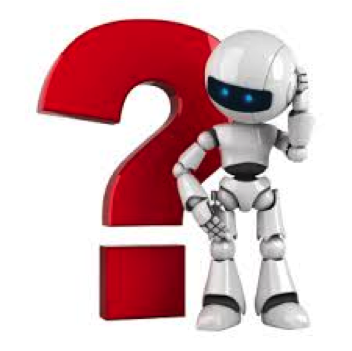
\includegraphics[width=.3\textwidth]{robot_quest.png}
\end{frame}

\begin{frame}
  \frametitle{A simple example}
  \begin{tabular}{c|c}
    Real world & Abstract model \\ \\ 
\begin{tikzpicture}[scale=1.7]
  \onslide<-13>{\draw[thick] (0,0) rectangle (2,2);}
  \onslide<14>{\draw[-,thick] (2,0) -- (0,0) -- (0,2) -- (2,2) -- (2,1);}
  \onslide<15>{\draw[thick] (0,0) rectangle (3,2);}
  \draw[thin,dashed] (0,1) -- (2,1);
  \draw[thin,dashed] (1,0) -- (1,2);
  \onslide<15>{\draw[thin,dashed] (2,0) -- (2,2);}
  \onslide<15>{\draw[thin,dashed] (2,1) -- (3,1);}  
  \onslide<8-> {\draw[thick] (1,1) -- (1,2);}
  \onslide<8-> {\draw[thick] (1,1) -- (2,1);}
  \onslide<1>{\node at (.5,.5) {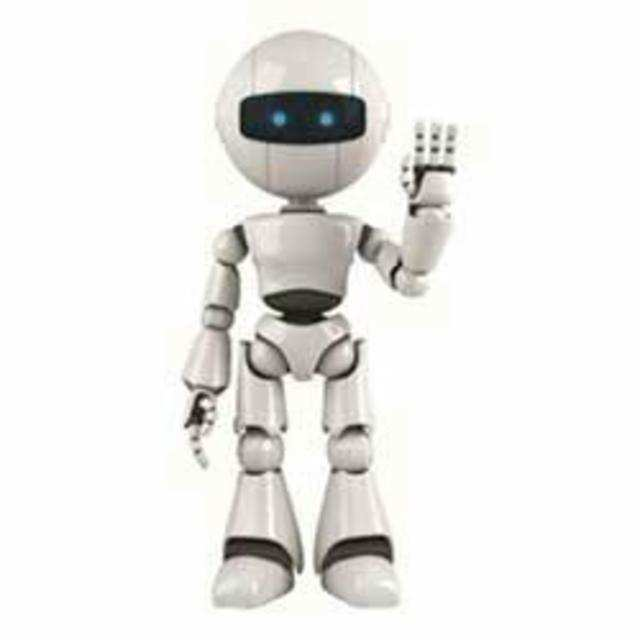
\includegraphics[width=1.3cm]{robot.jpg}};}
  \onslide<2>{\node at (1.5,.5) {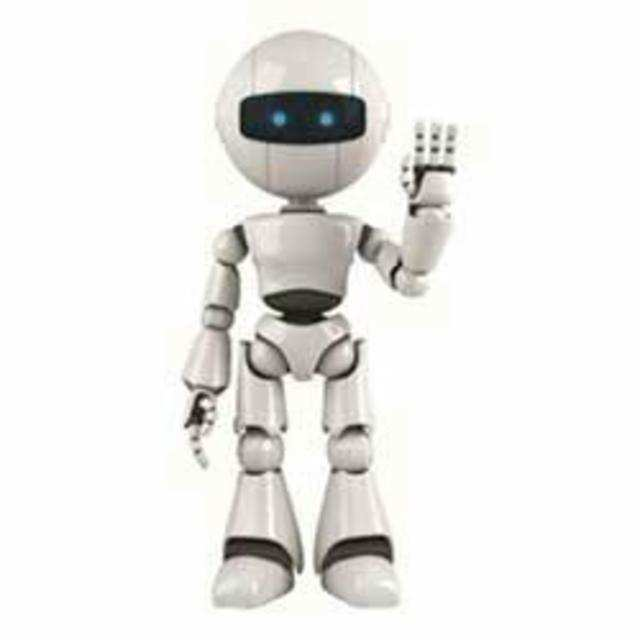
\includegraphics[width=1.3cm]{robot.jpg}};}
  \onslide<3>{\node at (1.5,1.5) {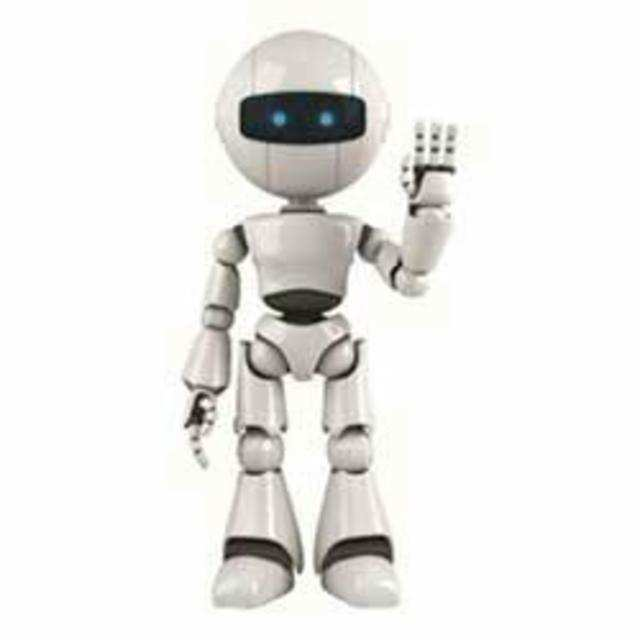
\includegraphics[width=1.3cm]{robot.jpg}};}
  \onslide<4>{\node at (.5,1.5) {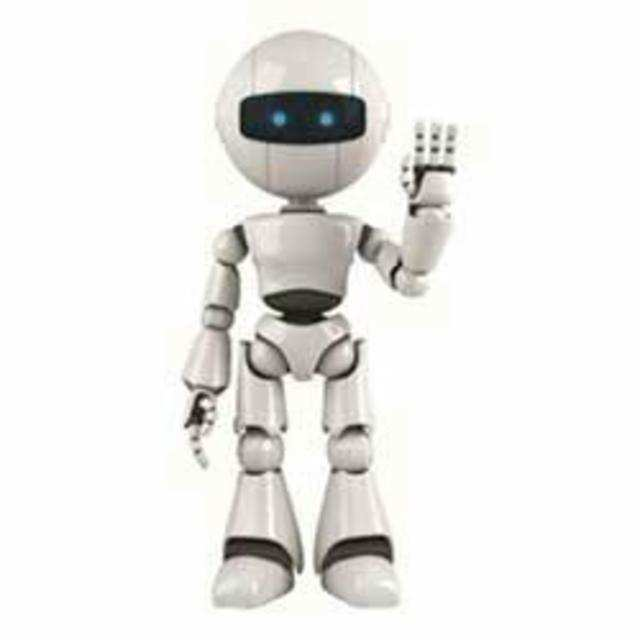
\includegraphics[width=1.3cm]{robot.jpg}};}
  \onslide<5>{\node at (.5,.5) {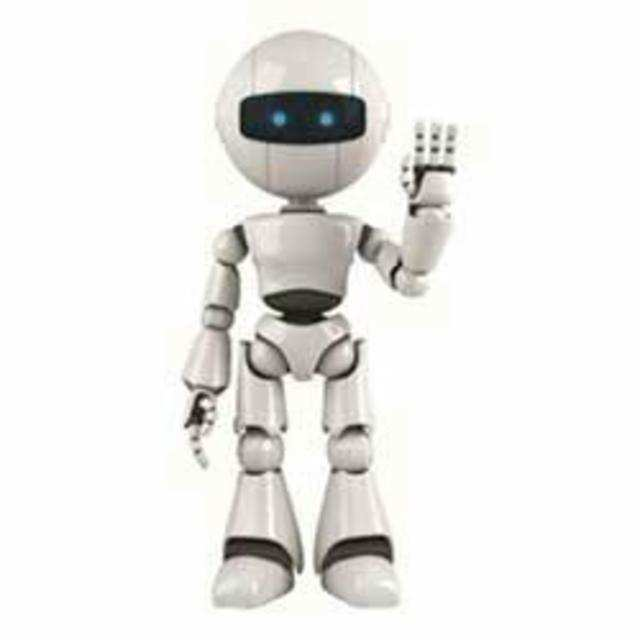
\includegraphics[width=1.3cm]{robot.jpg}};}
  \onslide<6-9>{\node at (.5,1.5) {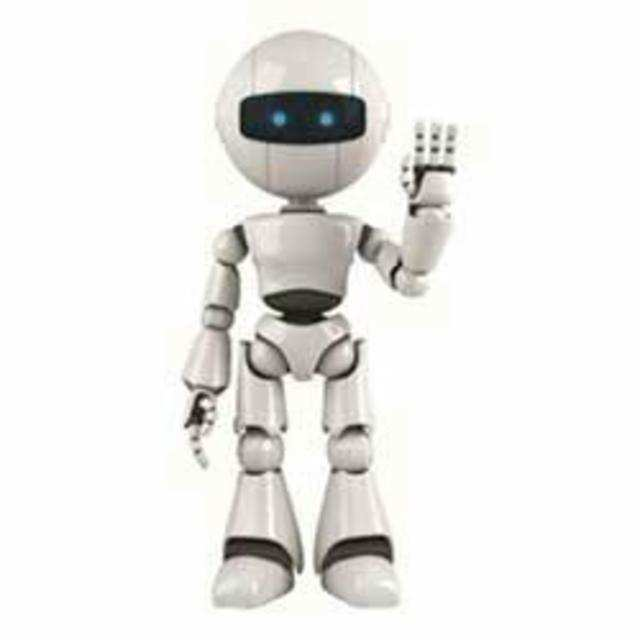
\includegraphics[width=1.3cm]{robot.jpg}};}
  \onslide<10>{\node at (.5,.5) {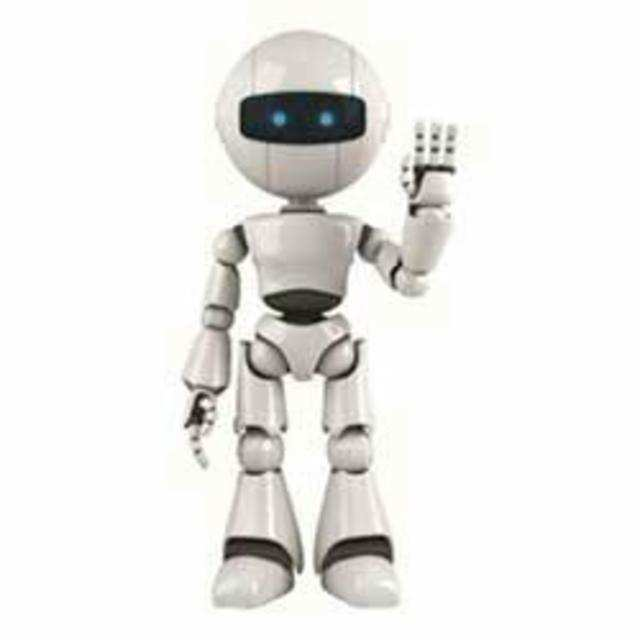
\includegraphics[width=1.3cm]{robot.jpg}};}
  \onslide<11>{\node at (1.5,.5) {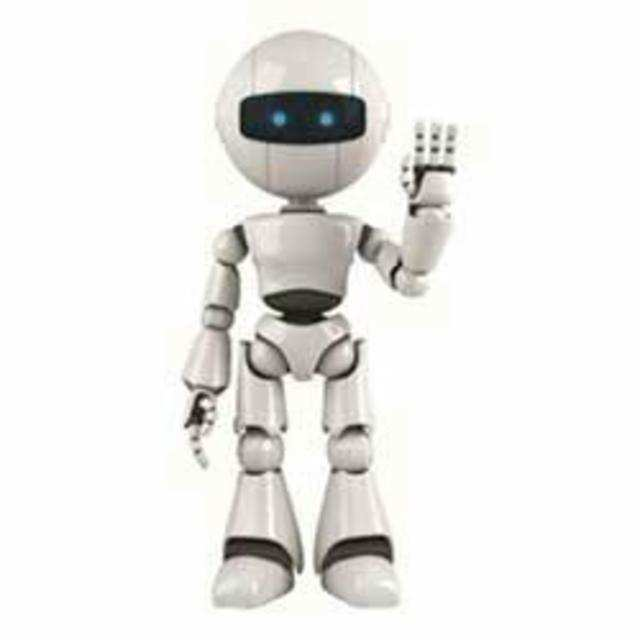
\includegraphics[width=1.3cm]{robot.jpg}};}
  \onslide<12>{\node at (2.5,.5) {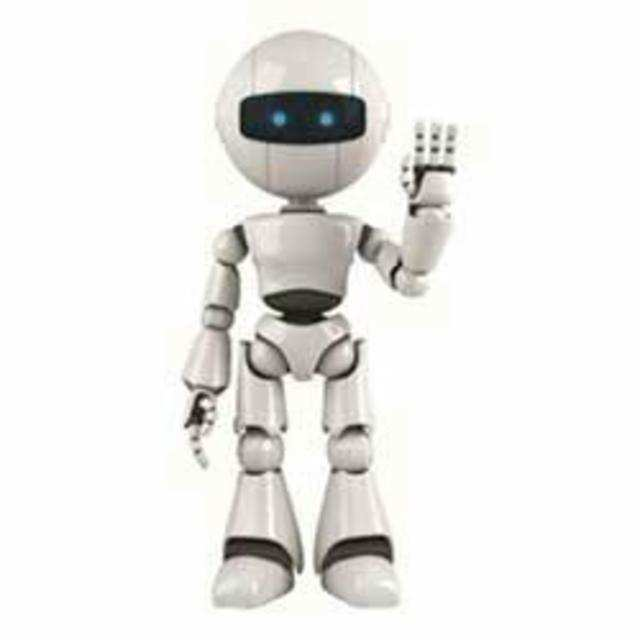
\includegraphics[width=1.3cm]{robot.jpg}};}    
  \onslide<13>{\node at (2.5,.5) {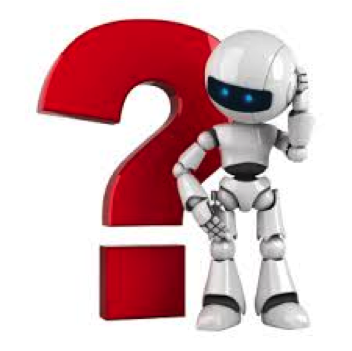
\includegraphics[width=1.3cm]{robot_quest.png}};}
  \onslide<14>{\node at (2.5,.5) {
\includegraphics[width=1.3cm]{robot_learned.jpg}};}
  \onslide<15>{\node at (1.5,1.5) {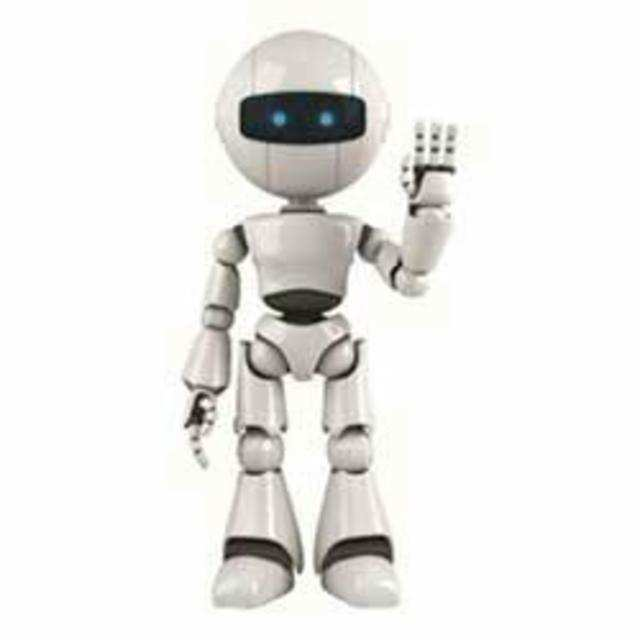
\includegraphics[width=1.3cm]{robot.jpg}};}      
\end{tikzpicture} & 
\begin{tikzpicture}[scale=2.2,auto,->]
  \node[state] (s11) {$s_{11}$};
  \only<1,5,10>{\node[fill=blue!20,state] {$s_{11}$};}
  \node[state,above = of s11] (s12) {$s_{12}$};
  \only<4,6-9>{\node[fill=blue!20,state,above = of s11] {$s_{12}$};}  
  \node[state,right = of s11] (s21) {$s_{21}$};
  \only<2,11>{\node[fill=blue!20,state,right = of s11] {$s_{21}$};}
  \node[state,above = of s21] (s22) {$s_{22}$};
   \only<3,15>{\node[fill=blue!20,state,above = of s21] {$s_{22}$};}
   \onslide<14->{\node[fill=red!20,state,right = of s21] (s31) {$s_{31}$};}
   \onslide<15>{\node[fill=red!20,state,right = of s22] (s32) {$s_{32}$};}
\onslide<2->{\path (s11) edge [bend left] node {$e$} (s21);}
\onslide<3-8>{\path (s21) edge [bend left] node {$n$} (s22);}
\onslide<4-8>{\path (s22) edge [bend left] node {$w$} (s12);}
\onslide<5->{\path (s12) edge [bend left] node {$s$} (s11);}
\onslide<6->{\path (s11) edge [bend left] node {$n$} (s12);}
\onslide<7->{\path (s21) edge [bend left] node {$w$} (s11);}
\onslide<7-8>{\path (s12) edge [bend left] node {$e$} (s22);}
\onslide<7-8>{\path (s22) edge [bend left] node {$s$} (s21);}
\onslide<14->{\path[red] (s21) edge [bend left] node {$e$} (s31);}
\onslide<15>{\path[red] (s31) edge [bend left] node {$w$} (s21);}
\onslide<15>{\path[red] (s31) edge [bend left] node {$n$} (s32);}
\onslide<15>{\path[red] (s32) edge [bend left] node {$s$} (s31);}
\onslide<15>{\path[red] (s32) edge [bend left] node {$w$} (s22);}
\onslide<15>{\path[red] (s22) edge [bend left] node {$e$} (s32);}
\end{tikzpicture}
  \end{tabular}
\end{frame}

\begin{frame}\small
  \frametitle{Overview}
  \begin{block}{Abstract world and real world}
   While an agent can conveniently plan at the
  \alert{abstract level}, it perceives the world and acts in it through
  sensors and actuators that work with data in a \alert{continuous world},
  typically represented with variables on real numbers.
  \end{block}\pause 
  \begin{block}{Planning and Learning}
      Most of the works on planning and learning assumes
      \begin{enumerate}[(i)]
      \item an abstract planning domain in which the set of states is fixed;
      \item the mapping between the observations
        from the real word and the states is implicit and fixed
      \end{enumerate}
    the focus is on \alert{learning the transitions} between
    states.
  \end{block}\pause 
  \begin{block}{Unexpected observations}
    There may be situations in which the agent perceives 
    {\color {red} data which are not compatible} with any of the states of its abstract
    model. 
%A revision of the set of states and the mapping between
%  observations and states is required in this case. 
  \end{block}
\end{frame}

\begin{frame}
  \frametitle{Objective}
  
A formal framework in which

\begin{enumerate}[(i)]
    \item  the agent can {\color {red} learn dynamically new states} of the planning domain;
    \item the {\color {red} mapping} between abstract {\color {red} states} and the {\color {red} perception} from the real world, represented by {\color {red} continuous variables}, is part of the planning domain; 
    \item
    such {\color {red} mapping is learned} and updated along the “life” of the agent.  
\end{enumerate}

\end{frame}

\begin{frame}

\frametitle{Approach}
 
We provide a formal framework in which
%the agent can learn dynamically new states of the planning domain and
%mapping from real world observations to states. while planning and
%executing.
\begin{enumerate}[(i)]
  \item    We model agent's perception of the real world by a
{\color {red} 
 \emph{perception function}} that returns {\color {red} the likelihood of observing some continuous data being in a state} of the domain.

Intuitively, when the likelihood is too low for all
the existing states, a new state is created;
\pause
\item We define an {\color {red} algorithm that interleaves planning, acting, and learning}. 
It is able to discover that the abstract model is not
coherent with the real world.  
%While planning and acting, 
%the algorithm 
It {\color {red} updates} both the set of {\color {red} states} and the {\color {red} perception function} of the
planning domain.
\end{enumerate}  
\end{frame}

\begin{frame}
\frametitle{Planning Domains with  Perception Functions}

\begin{itemize}
\item 
Deterministic Planning Domain: $\PD=\left<S,A,\gamma\right>$
\item 
State transition function: $\gamma: S \times A \rightarrow S$
\item
Planning Problem: $\PP= \left<\PD,s_0,S_g\right>$
\item
A Plan $\pi$ is a policy:
partial function from $\pi: S  \rightharpoonup A$.  
\pause
\item
{\color {red} Perception Function:  $f:\R^n\times S\rightarrow R^+$}, where $f(\bx,s) = p(\bx|s)$ is a join PDF on $\R^n\times S$\\
{\color {red} $f(\bx,s)$ is the likelihood of observing $\bx$ being in a state
$s$.}
\end{itemize}  
\end{frame}

\begin{frame}
  \frametitle{Simple univariate perception function}

  \begin{example}
    \begin{itemize}
    \item $S=\{{\color{blue}s_1},{\color{red}s_2}\only<5>{,s_{new}}\}$
    \item $\color{blue}f(x,s_1) = \N(\mu=2,\sigma=0.21)$
    \item $\color{red}f(x,s_2) = \N(\mu=10,\sigma=0.21)$
    \only<5>{\item $f(x,s_{new}) = \N(\mu=7,\sigma=0.21)$}           
    \end{itemize}
  \end{example}
  
  
\begin{tikzpicture}
\begin{axis}[every axis plot post/.append style={
  mark=none,domain=-2:14,samples=50,smooth},
  width=\textwidth,
  height=0.5\textwidth,
  axis x line*=bottom, 
  axis y line*=left,
  ymax = 0.34]
  \addplot {gauss(2,1.5)} node [pos=.25,above] {$f(x,s_1)$};
  \addplot {gauss(10,1.5)} node [pos=.7 5,above] {$f(x,s_2)$};;
  \addplot {.1} node[above] {$\epsilon$};
  \only<2>{\node at (1,0) {$\bullet$};}
  \only<2>{\node[blue] at (1,0.21) {$\bullet$};}  
  \only<2>{\draw[dotted] (1,0) -- (1,0.21);}
  \only<3>{\node at (9,0) {$\bullet$};}
  \only<3>{\node[red] at (9,0.21) {$\bullet$};}  
  \only<3>{\draw[dotted] (9,0) -- (9,0.21);}
  \only<4>{\node at (7,0) {$\bullet$};}
  \only<4>{\node[red] at (7,0.032) {$\bullet$};}  
  \only<4>{\draw[dotted] (7,0) -- (7,0.032);}
  \only<5>{\addplot {gauss(7,1.5)}node [pos=.55,above] {$f(x,s_{new})$};}
\end{axis}
\end{tikzpicture}

\begin{tikzpicture}
  \only<2>{\node[blue,left] at (0,0) {$s_1=\argmax_{s\in\{s_1,s_2\}}f(1.0,s)$ and $f(1,0,s_1)\geq \epsilon$};}
  \only<3>{\node[red,left] at (0,0) {$s_2=\argmax_{s\in\{s_1,s_2\}}f(9.0,s)$ and $f(9,0,s_2)\geq \epsilon$};}
  \only<4>{\node[left] at (0,0) {$s_2=\argmax_{s\in\{s_1,s_2\}}f(7.0,s)$ and $f(7,0,s_2) < \epsilon$};}  
  \only<5>{\node[left] at (0,0) {$s_{new}=\argmax_{s\in\{s_1,s_2,s_{new}\}}f(7.0,s)$ and $f(7,0,s_{new}) \geq \epsilon$};}  
\end{tikzpicture}
\end{frame}


\begin{frame}
\frametitle{The Planning, Acting, and Learning (PAL) Algorithm}
  \scalebox{.7}{
  \begin{algorithm}[H]
\caption{\sc PlanActLearn - PAL}
\label{PlanActLearn}  
 \begin{algorithmic}[1] 
   \REQUIRE $\PP=\left<\PDdef,s_0,S_g,{\color {red} f}\right>$ \COMMENT{
   {\color {red}  A planning problem with a perception function}}
   \REQUIRE{$p_{init}(\cdot)$ initialization for $f(\cdot,s)$}
   \STATE{$\T\gets\langle\rangle$}\ \ \ \ \ \COMMENT{The empty history of transitions}
   \STATE{$\O\gets\langle\rangle$}\ \ \ \ \ \COMMENT{The empty history of observations}
\pause
   \WHILE{$s_0\not\in S_g$}
   \STATE {\color {red} $\pi\gets plan(\PP)$}
\pause
   \WHILE {$\pi(s_0)$ is defined and $\gamma$ has not been changed} 
   \STATE {\color {red} $\bx\gets act(\pi(s_0))$} 
   \STATE {\color {red} $s'_0 \gets \arg\!\max_{s\in S}f(\bx,s)$}
   \IF{{\color {red} $f(\bx,s_0') < (1-\epsilon)\cdot\max p_{init}(\cdot)$}}
   
   \STATE {\color {red} $s'_0\gets s_{new}$}
   \STATE $S\gets S\cup\{s_{new}\}$
   \STATE $f(\cdot,s_{new}) = p_{init}(\cdot)$
   \ENDIF
\pause
   \STATE{$\T \gets append(T,\left<s_0,\pi(s_0),s_0'\right>)$}
   \COMMENT{extend the transition history with the last one}
   \STATE{$\O \gets append(\O,\left<s'_0,\bx\right>$)}
   \COMMENT{extend the observation history with the last one}
\pause
   \STATE {\color {red} $\gamma \gets \updgamma(\gamma,\T)$}
           \STATE {\color {red} $f \gets \updf(f,\O)$}
   \STATE $ s_0 \gets s'_0$
   \ENDWHILE   
   \ENDWHILE
\end{algorithmic}
\end{algorithm}}
\end{frame}

\begin{frame} 
  \frametitle{Updating Transitions: $\updgamma$ Example}

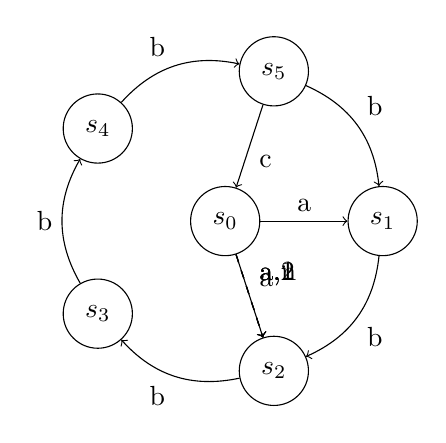
\begin{tikzpicture}[baseline=(s0.base),auto,->]
  \node[state, onslide={<1,7,11>{highlight}}] (s0) {$s_{0}$};
  \node[state, onslide={<2>{highlight}}] at (0:2) (s1) {$s_{1}$};
  \node[state, onslide={<3,8,12,13>{highlight}}] at (-1*72:2) (s2) {$s_{2}$};
  \node[state, onslide={<4,9>{highlight}}] at (-2*72:2) (s3) {$s_{3}$};
  \node[state, onslide={<5>{highlight}}] at (-3*72:2) (s4) {$s_{4}$};
  \node[state, onslide={<6,10>{highlight}}] at (-4*72:2) (s5) {$s_{5}$};
  \draw<-13> (s0) to node {a} (s1);
  \draw<14> (s0) to node {a} (s2);  
  \draw<8-11>[dashed] (s0) to node {a,1} (s2);
  \draw<12>[dashed] (s0) to node {a,2} (s2);
  \draw<13>[dashed] (s0) to node {a,n} (s2);      
  \draw (s1) to[bend left] node {b} (s2);
  \draw (s2) to[bend left] node {b} (s3);
  \draw (s3) to[bend left] node {b} (s4);
  \draw (s4) to[bend left] node {b} (s5);
  \draw (s5) to[bend left] node {b} (s1);  
  \draw (s5) to node {c} (s0);
\end{tikzpicture}
\begin{tabular}{rccc}
iter   &  Source & action & Target \\ \hline \pause
  1 &  $s_0$  & $a$ & $s_1$ \pause \\
  2 &  $s_1$  & $b$ & $s_2$ \pause \\
  3 &  $s_2$  & $b$ & $s_3$ \pause \\
  4 &  $s_3$  & $b$ & $s_4$ \pause \\  
  5 &  $s_4$  & $b$ & $s_5$ \pause \\
  6 &  $s_5$  & $c$ & $s_0$ \pause \\
  7 &  $s_0$  & $a$ & $s_2$ \pause \\
  8 &  $s_2$  & $b$ & $s_3$ \\
  9 &  $s_3$  & $b$ & $s_4$ \\
  10 &  $s_4$  & $b$ & $s_5$ \pause \\
  11 &  $s_5$  & $c$ & $s_0$ \pause \\
  12 &  $s_0$  & $a$ & $s_2$ \pause \\
  \vdots & \\ 
  \dots &  $s_0$  & $a$ & $s_2$ \\ 
\end{tabular}
\end{frame}

\begin{frame} 
  \frametitle{Updating Transitions: $\updgamma$} 

\begin{itemize}
\item[$\bullet$] 
$\updgamma$ decides whether and how to update the transition function.
\pause
\item[$\bullet$]
After executing $a$, the agent perceives $\bx$. 
\pause
\item[$\bullet$]
Suppose that $\argmax_{s}(f(\bx,s)) \neq \gamma(a,s)$
\pause
\item[$\bullet$]
This means that the most likely reached state is different from the predicted state.
\pause
\item[$\bullet$]
Then the execution of an action leads to an unexpected state
\pause
\item[$\bullet$]
We have two options: either change $\gamma$ with the new transition or not.
\pause
\item[$\bullet$]
{\color {red} Whether we change it or not depends on how much we trust the current model (that has been given or learned so far)}
\end{itemize}
\end{frame}



\begin{frame} 
  \frametitle{Updating Transitions: A proposal} 

$\updgamma(\gamma,\T)(s,a)=s'$  where $s'$ is \emph{one element}
of the set

$$
\{\argmax_{s'\in S}\left(\alpha\cdot\mathbb{1}_{s'=\gamma(s,a)}+
    (1-\alpha)\cdot|\{i\mid \T_i=\left<s,a,s'\right>\}|
\right)\}
$$

with $\alpha\in[0,1]$.

\pause
\vspace{1cm}
Notice that,
\begin{itemize}
\item[$\bullet$] 
if {\color {red} $\alpha = 1$}, we are extremely cautious, we strongly believe in our
model of the world, and we never change the transition $\gamma$.
\pause
\item[$\bullet$] 
if {\color {red} $\alpha = 0$}, we are extremely impulsive, we do not trust our model,
and just one evidence makes us to change the model.
\pause
\item[$\bullet$] 
if {\color {red} $\alpha \in (0,1)$}, depending on the value of
$\alpha$, we need more or less evidence to change the planning
domain.
\end{itemize}
\end{frame}


\begin{frame} 
  \frametitle{Updating the Perception Function: Example } 

\begin{tikzpicture}
\begin{axis}[every axis plot post/.append style={
  mark=none,domain=-2:14,samples=30,smooth},
  width=\textwidth,
  height=0.5\textwidth,
  axis x line*=bottom, 
  axis y line*=left,
  ymax = 0.34]

  \only<1-2>{\addplot[blue]{gauss(2,1.5)} node [pos=.5,above right] {$f(x,s_1)$};}
  \only<3->{\addplot[blue,dotted] {gauss(2,1.5)};}
  \only<3-4>{\addplot[blue]{gauss(1.8,1.5)} node [pos=.5,above right] {$f(x,s_1)$};}
  \only<5->{\addplot[blue,dotted]{gauss(1.8,1.5)};}
  \only<5-6>{\addplot[blue]{gauss(1.7,1.5)} node [pos=.5,above right] {$f(x,s_1)$};}
  \only<7->{\addplot[blue,dotted]{gauss(1.7,1.5)};}
  \only<7-8>{\addplot[blue]{gauss(1.1,1.5)} node [pos=.5,above right] {$f(x,s_1)$};}
  \only<9->{\addplot[blue,dotted]{gauss(1.1,1.5)};}
  \only<9-10>{\addplot[blue]{gauss(1.3,1.5)} node [pos=.5,above right] {$f(x,s_1)$};}
  \addplot[red] {.1} node[above] {$\epsilon$};
  \draw<2->[dashed] (.75,0) -- (.75,4);
  \node<2-> at (.75,-.02) {$x_0$};
  \draw<4->[dashed] (1.5,0) -- (1.5,4);  
  \node<4-> at (1.5,-.02) {$x_1$};
  \draw<6->[dashed] (0,0) -- (0,4);
  \node<6-> at (0,-.02) {$x_2$};
  \draw<8->[dashed] (2.5,0) -- (2.5,4);
  \node<8-> at (2.5,-.02) {$x_3$};  
\end{axis}
\end{tikzpicture}
\end{frame}

\begin{frame} 
  \frametitle{Updating the Perception Function} 

\begin{itemize}
\item[$\bullet$]
The update of the perception function is based on the 
{\color {red} current
perception function $f(\bx,s)$} and 
{\color {red} the set of observations $\O$} ($\O \gets append(\O,\left<s,\bx\right>$). 
\pause
\item[$\bullet$]
We suppose 
{\color {red} $f$ is parametric on $\prm=\left<\theta_1,\dots,\theta_k\right>$}
(normal distribution: 
{\color {red} 
$\theta_1=\bmu$ and $\theta_2=\bSigma$}) 
\pause
\item[$\bullet$]
We have a new observation $\left<\bx,s\right>$ and a set of previous
observations $\O(s)=\left<\bx^{(0)},\dots, \bx^{(k)}\right>$ \pause
\item[$\bullet$]
We have to 
{\color {red} 
update the parameters $\prm_s$} of
the perception function $f(\cdot,s)$ in order to
{\color {red}  maximize the likelihood} of the entire set of observations extended
with the new observation.
\pause
\item[$\bullet$]
Also in this case the agent can be more or less
careful in the revision: Parameter 
{\color {red}  $\beta\in[0,1]$} -  the higher the value of $\beta$ the more careful the agent is in the revision.
\end{itemize}

\end{frame}

\begin{frame} 
  \frametitle{Updating the Perception Function: A proposal} 

Let $f(\bx,s) = p(\bx|s,\prm_s)$. We define
$\updf(f,\O)(\bx,s)$ as 
$p(\bx\mid s,\prm'_s))$
where: 
\begin{align}\small
  \label{eq:update-f}
  \prm'_s & = \beta\cdot\prm_s+(1-\beta)\cdot
            \argmax_{\prm''} \mathcal{L}(\prm_s'',\O(s),\bx,s)
\end{align}
where 
$\mathcal{L}(\prm,\bx^{(1)},\dots,\bx^{(n)},s)$ 
is the likelihood of the 
parameters $\prm$ for the observations $\bx^{(1)},\dots,\bx^{(n)}$,
defined as: 
\begin{align}
  \label{eq:max-like-prm}
\mathcal{L}(\prm,\bx^{(1)},\dots,\bx^{(n)},s) & = 
  \prod_{i=1}^nP(\bx^{(i)}|s,\prm)
\end{align}

%\begin{itemize}
%\item[$\bullet$]
%Equation \eqref{eq:update-f} defines the parameters
%$\prm'_s$ of the updated perception function for a state $s$ as a
%convex combination, based on the parameter $\beta$, of the parameters
%of the previous perception functions for $s$, i.e., $\prm_s$ and the
%parameters $\prm''$ that maximise the likelihood of the past and
%current observations about state $s$ (equation
%\eqref{eq:max-like-prm}).  
%\end{itemize}

%An efficient procedure for incremental
%estimation of the second term of \eqref{eq:update-f}, is described in
%\cite{bishop2006}. 


In case of Multivariate Gaussian distribution:
\begin{align*}
  \bmu'_s & = \beta\cdot\bmu_s+(1-\beta)(\bmu_s + \Delta\bmu_s) \\
  \bSigma'_s & = \beta\cdot\bSigma_s+(1-\beta)(\bSigma_s + \Delta\bSigma_s) \\
\end{align*}

\vspace*{-1cm}
where $\Delta\bmu_s=\frac{1}{|\O(s)|}(\bx-\bmu_s)$
and $\Delta\bSigma^2_s = \frac{1}{|O(s)|}(\bx-\bmu_s')^2 +
\frac{|O(s)|-1}{|O(s)|}(\Delta\bmu_s^2-2\bmu_s\Delta\bmu_s) -\frac{1}{|O(s)|}\bSigma^2_s$.

%Concerning the parameter $\beta\in[0,1]$, it plays the similar role
%as $\alpha$ in the case of the revision of the transition function.
%It balances the update depending on whether the agent is cautious or impulsive
%about the current perception function, and the new perceptions. 


\end{frame}


\begin{frame}
  \frametitle{A simple example}
  \begin{center}
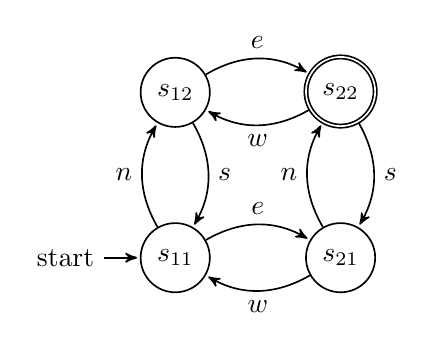
\begin{tikzpicture}[->,>=stealth',shorten >=1pt,auto,node distance=1.2cm,
                    semithick,  baseline=(current bounding box.center)]
\node[initial,state] (s11) {$s_{11}$};
\node[state,above = of s11] (s12) {$s_{12}$};
\node[state,right = of s11] (s21) {$s_{21}$};
\node[state,accepting,above = of s21] (s22) {$s_{22}$};
\path (s11) edge [bend left] node {$e$} (s21)
            edge [bend left] node {$n$} (s12)
%            edge [loop below] node {$s,w$} (s11)
      (s12) edge [bend left] node {$e$} (s22)
            edge [bend left] node {$s$} (s11)
%            edge [loop left] node {$n,w$} (s12)
      (s21) edge [bend left] node {$w$} (s11)
            edge [bend left] node {$n$} (s22)
%            edge [loop right] node {$s,e$} (s21)
      (s22) edge [bend left] node {$w$} (s12)
%            edge [loop right] node {$n,e$} (s22)
            edge [bend left] node {$s$} (s21);
          \end{tikzpicture} 
\begin{tikzpicture}[scale=.7,baseline=(current bounding box.center)]
  \begin{axis}[view={0}{90},
    colormap/hot,
    xmin = 0,
    xmax = 3,
    ymin = 0,
    ymax = 2,
    axis equal image,
    samples=10,
    domain=0:2,
    y domain=0:2,
    ]
   \def\centerx{.5}
   \def\centery{.5}
    \addplot3[contour gnuplot,domain=-2:6,domain y=-5:3] 
        {10*exp(-10*( (x-\centerx)^2 + (y-\centery)^2)/3 )};
   \def\centerx{1.5}
   \def\centery{.5}
    \addplot3[contour gnuplot,domain=-2:6,domain y=-5:3] 
        {10*exp(-10*( (x-\centerx)^2 + (y-\centery)^2)/3 )};
   \def\centerx{1.5}
   \def\centery{1.5}
    \addplot3[contour gnuplot,domain=-2:6,domain y=-5:3] 
        {10*exp(-10*( (x-\centerx)^2 + (y-\centery)^2)/3 )};
   \def\centerx{.5}
   \def\centery{1.5}
    \addplot3[contour gnuplot,domain=-2:6,domain y=-5:3] 
        {10*exp(-10*( (x-\centerx)^2 + (y-\centery)^2)/3 )};
      \end{axis}
    \end{tikzpicture}
       
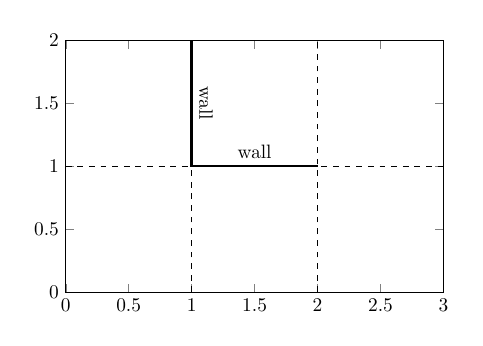
\begin{tikzpicture}[scale=.7,baseline=(current bounding box.center)]
  \begin{axis}[view={0}{90},
    xmin = 0,
    xmax = 3,
    ymin = 0,
    ymax = 2,
    axis equal image,
    domain=0:2,
    y domain=0:2]
    \draw[very thick] (1,2) -- node[sloped,above]{wall} (1,1) -- node[auto]{wall}(2,1);
    \draw[thin,dashed] (0,1) -- (3,1);
    \draw[thin,dashed] (1,0) -- (1,2);
    \draw[thin,dashed] (2,0) -- (2,2);    
  \end{axis}
\end{tikzpicture}
\end{center}
\end{frame}

\begin{frame}
  \frametitle{A simple example}
  \begin{center}
  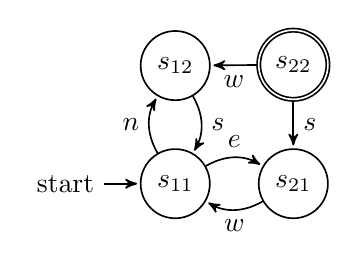
\begin{tikzpicture}[->,>=stealth',shorten >=1pt,auto,node distance=.6cm,
                    semithick,  baseline=(current bounding box.center)]
                    \node[initial,state] (s11) {$s_{11}$};
\node[state,above = of s11] (s12) {$s_{12}$};
\node[state,right = of s11] (s21) {$s_{21}$};
\node[state,accepting,above = of s21] (s22) {$s_{22}$};
\path (s11) edge [bend left] node {$e$} (s21)
            edge [bend left] node {$n$} (s12)
      (s12) edge [bend left] node {$s$} (s11)
      (s21) edge [bend left] node {$w$} (s11)
      (s22) edge node {$w$} (s12)
            edge node {$s$} (s21);            
     \end{tikzpicture} 
%
\begin{tikzpicture}[scale=.7,baseline=(current bounding box.center)]
  \begin{axis}[view={0}{90},
    colormap/hot,
    xmin = 0,
    xmax = 3,
    ymin = 0,
    ymax = 2,
    axis equal image,
    samples=10,
    domain=0:2,
    y domain=0:2,
    ]
   \def\centerx{.5}
   \def\centery{.5}
    \addplot3[contour gnuplot,domain=-2:6,domain y=-5:3] 
        {10*exp(-10*( (x-\centerx)^2 + (y-\centery)^2)/3 )};
   \def\centerx{1.5}
   \def\centery{.5}
    \addplot3[contour gnuplot,domain=-2:6,domain y=-5:3] 
        {10*exp(-10*( (x-\centerx)^2 + (y-\centery)^2)/3 )};
   \def\centerx{1.5}
   \def\centery{1.5}
    \addplot3[contour gnuplot,domain=-2:6,domain y=-5:3] 
        {10*exp(-10*( (x-\centerx)^2 + (y-\centery)^2)/3 )};
   \def\centerx{.5}
   \def\centery{1.5}
    \addplot3[contour gnuplot,domain=-2:6,domain y=-5:3] 
        {10*exp(-10*( (x-\centerx)^2 + (y-\centery)^2)/3 )};
      \end{axis}
    \end{tikzpicture}
       
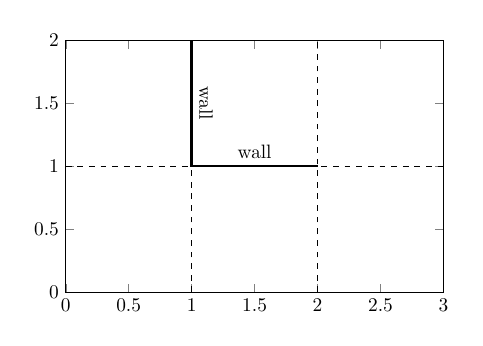
\begin{tikzpicture}[scale=.7,baseline=(current bounding box.center)]
  \begin{axis}[view={0}{90},
    xmin = 0,
    xmax = 3,
    ymin = 0,
    ymax = 2,
    axis equal image,
    domain=0:2,
    y domain=0:2]
    \draw[very thick] (1,2) -- node[sloped,above]{wall} (1,1) -- node[auto]{wall}(2,1);
    \draw[thin,dashed] (0,1) -- (3,1);
    \draw[thin,dashed] (1,0) -- (1,2);
    \draw[thin,dashed] (2,0) -- (2,2);    
  \end{axis}
\end{tikzpicture}
\end{center}
\end{frame}

\begin{frame}
  \frametitle{A simple example}
  \begin{center}
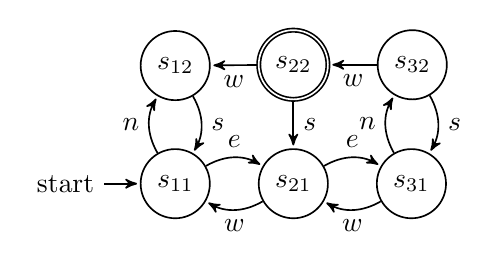
\begin{tikzpicture}[->,>=stealth',shorten >=1pt,auto,node distance=.6cm,
                    semithick,  baseline=(current bounding box.center)]
\node[initial,state] (s11) {$s_{11}$};
\node[state,above = of s11] (s12) {$s_{12}$};
\node[state,right = of s11] (s21) {$s_{21}$};
\node[state,accepting,above = of s21] (s22) {$s_{22}$};
\node[state,right = of s21] (s31) {$s_{31}$};
\node[state,right = of s22] (s32) {$s_{32}$};
\path (s11) edge [bend left] node {$e$} (s21)
            edge [bend left] node {$n$} (s12)
      (s12) edge [bend left] node {$s$} (s11)
%            edge [loop left] node {$n,w$} (s12)
      (s21) edge [bend left] node {$e$} (s31)
            edge [bend left] node {$w$} (s11)
%            edge [loop below] node {$s,n$} (s21)
      (s22) edge node {$w$} (s12)
            edge node {$s$} (s21)
      (s31) edge [bend left] node {$w$} (s21)
            edge [bend left] node {$n$} (s32)
%            edge [loop below] node {$s,e$} (s21)
      (s32) edge node {$w$} (s22)
%             edge [loop left] node {$n,e$} (s32)
            edge [bend left] node {$s$} (s31);
      \end{tikzpicture} 
%
\begin{tikzpicture}[scale=.6,baseline=(current bounding box.center)]
  \begin{axis}[view={0}{90},
    colormap/hot,
    xmin = 0,
    xmax = 3,
    ymin = 0,
    ymax = 2,
    axis equal image,
    samples=10,
    domain=0:2,
    y domain=0:2,
    ]
   \def\centerx{.5}
   \def\centery{.5}
    \addplot3[contour gnuplot,domain=-2:6,domain y=-5:3] 
        {10*exp(-10*( (x-\centerx)^2 + (y-\centery)^2)/3 )};
   \def\centerx{1.5}
   \def\centery{.5}
    \addplot3[contour gnuplot,domain=-2:6,domain y=-5:3] 
        {10*exp(-10*( (x-\centerx)^2 + (y-\centery)^2)/3 )};
   \def\centerx{1.5}
   \def\centery{1.5}
    \addplot3[contour gnuplot,domain=-2:6,domain y=-5:3] 
        {10*exp(-10*( (x-\centerx)^2 + (y-\centery)^2)/3 )};
   \def\centerx{.5}
   \def\centery{1.5}
    \addplot3[contour gnuplot,domain=-2:6,domain y=-5:3] 
        {10*exp(-10*( (x-\centerx)^2 + (y-\centery)^2)/3 )};
      \end{axis}
    \end{tikzpicture}
       
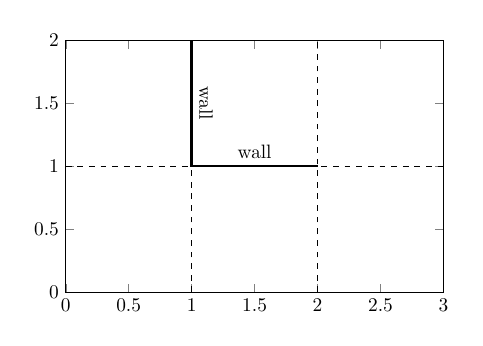
\begin{tikzpicture}[scale=.7,baseline=(current bounding box.center)]
  \begin{axis}[view={0}{90},
    xmin = 0,
    xmax = 3,
    ymin = 0,
    ymax = 2,
    axis equal image,
    domain=0:2,
    y domain=0:2]
    \draw[very thick] (1,2) -- node[sloped,above]{wall} (1,1) -- node[auto]{wall}(2,1);
    \draw[thin,dashed] (0,1) -- (3,1);
    \draw[thin,dashed] (1,0) -- (1,2);
    \draw[thin,dashed] (2,0) -- (2,2);    
  \end{axis}
\end{tikzpicture}
\end{center}
\end{frame}

\begin{frame}
\frametitle{Measuring the Coherence of the Model}
\footnotesize
\begin{itemize}
\item[$\bullet$] 
We represent the effects of executing the action $a$ in the real world with
$p_a(\bx'|\bx)$, i.e., the probability of measuring $\bx'$ after executing the action $a$.
\item[$\bullet$] 
We compare $p_a(\bx'|\bx)$ with $p(\bx'|s')$, 
the probability of observing $\bx'$ after the execution
of $a$ according to the agent's abstract model 
\item[$\bullet$] 
{\em KL divergence} 
$KL(p_a(\bx'|\bx)||p(\bx'|s'))$,
defined as: 
$$
\int_{\bx'}p_a(\bx'|\bx)\log\left(\frac{p_a(\bx'|\bx)}{p(\bx'|s')}\right)\:d\bx'
$$
\item[$\bullet$] 
{\em Divergence measure} 
\begin{align}
  \label{eq:coherence}
  \int_{\bx}\sum_{a\in
  A}\mathrm{KL}(p_a(\bx'|\bx)||p(\bx'|\gamma(a,s_{\bx})))\cdot p_A(\bx)\: d\bx
\end{align}
where $s_{\bx}=\argmax_{s\in  S}f(\bx,s))$ and $p_A(\bx)$ is a distribution of all the possible perceptions
that can be obtained by the agent following all the possible sequences
of actions, i.e., 
$$
p_A(\bx)=\sum_{\left<a_1.\dots,a_n\right>\in A^+}p_{a_n}(\bx|\bx^{(n-1)})\cdot\prod_{i=1}^{n-1}p_{a_i}(\bx^{(i)}|\bx^{(i-1)})
$$
\def\ba{\mathbf{a}}
%
where $A^+$ is the set of finite non empty sequences of actions in $A$
and $\bx^{(0)}$ is the perception of the agent in the initial state. 
\end{itemize}

\end{frame}

\begin{frame}
\frametitle{Measuring the Coherence of the Model}
\footnotesize
We estimate \eqref{eq:coherence} by random walk sampling method. Starting
from an initial observation $\bx^{(0)}$ we generate $N$ random
walks ${\bf a}_1,\dots,{\bf a}_N$, 
%
with
${\bf a}_i=\langle a_{i,1},\dots,a_{i,n_i}\rangle$ and sample $\bx^{(i)}$
from $\prod_{j=1}^{n_i}p_{a_{ij}}(\bx_{j}|\bx_{j-1})$. 
We approximate \eqref{eq:coherence} with
\begin{align}
  \label{eq:coherence-approx}
\frac{1}{N}\sum_{k=1}^N\sum_{a\in A}\mathrm{KL}(p_a(\bx'|\bx^{(k)})|| p(\bx'|\gamma(a,s^{(k)})))
\end{align}
where $s^{(k)} = \argmax_{s\in S}f(\bx^{(k)},s)$ for $1\leq k \leq
n$. 
In our specific example, since we are working with Gaussian
distributions, we have that 
%
$p_a(\bx'|\bx) =
\N(\bmu=a(\bx),\bSigma=\bSigma_a)$,
%
where $a(\bx)$ 
is some real function that maps  
$\bx$ in the expected value $a(\bx)$ after performing the action $a$, and $\bSigma_a$ is the model of the noise of the
sensors/actuators associated to $a$. For instance, in the 6 room example:
$$
e(\langle x,y\rangle)=
\begin{cases}
  \langle x+1,y\rangle & \parbox[t]{.3\textwidth}{If there are no walls
    between \\ $\left<x,y\right>$ ad $\left<x+1,y\right>$} \\
    \langle x,y\rangle & \mbox{Otherwise}
  \end{cases}
  $$
Furthermore, the KL divergence of Multivariate Gaussians can be
computed analytically. 

% using the following equation 
% \begin{equation}
%   \begin{split}
% & \frac{1}{2}\biggl( 
%   \log\frac{|\bSigma_{\gamma(a,s)}|}
%     {|\bSigma_{a}|}-d+tr(\bSigma_{\gamma(a,s)}^{-1}\bSigma_{a})
%      \\
%     &  \quad +(\bmu_{\gamma(a,s)}-a(\bx))^{\mathsf{T}}\bSigma_{\gamma(a,s)}^{-1}(\bmu_{\gamma(a,s)}-a(\bx))\biggr)
% \end{split}
% \end{equation}
% where $d$ is the dimension of $\bx$.

\end{frame}
    
\begin{frame}
\frametitle{Experimental Evaluation}
\scalebox{0.7}{
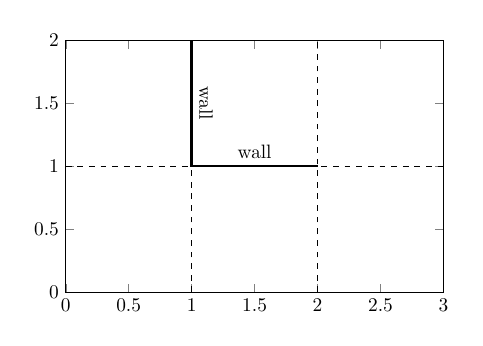
\begin{tikzpicture}[scale=.7,baseline=(current bounding box.center)]
  \begin{axis}[view={0}{90},
    xmin = 0,
    xmax = 3,
    ymin = 0,
    ymax = 2,
    axis equal image,
    domain=0:2,
    y domain=0:2]
    \draw[very thick] (1,2) -- node[sloped,above]{wall} (1,1) -- node[auto]{wall}(2,1);
    \draw[thin,dashed] (0,1) -- (3,1);
    \draw[thin,dashed] (1,0) -- (1,2);
    \draw[thin,dashed] (2,0) -- (2,2);    
  \end{axis}
\end{tikzpicture}
}

\begin{table}[t]\footnotesize
\centering
\def\toprule{\hline}
\def\midrule{\hline\hline}
\def\bottomrule{\hline}
\tabcolsep=3pt
\begin{tabular}{|l|l|r|r|r|r|r|r|r|r|r|}
\toprule
$\alpha$ & $\beta$ & 
\multicolumn{3}{|c|}{$\epsilon=0.0$} & 
\multicolumn{3}{|c|}{$\epsilon=0.5$} & 
\multicolumn{3}{|c|}{$\epsilon=1.0$} \\  \cline{3-11}
& & $|S|$ & \%lrn & \%G & 
$|S|$ & \%lrn & \%G & 
$|S|$ & \%lrn & \%G \\ \midrule
0.0 & 0.0 &          21.6 &        0.49 &           1.0 & 
                      6.0 &        0.72 &           0.7 & 
                      4.0 &       -4.71 &           0.1 \\
    & 0.5 &          24.7 &        0.50 &           0.9 & 
                      5.9 &        0.72 &           0.8 & 
                      4.0 &       -0.41 &           0.9 \\
    & 1.0 &          20.2 &        0.54 &           0.9 & 
                      5.9 &        0.72 &           0.7 & 
                      4.0 &        0.18 &           0.9 \\ 
0.5 & 0.0 &          25.8 &        0.19 &           1.0 & 
                      5.9 &        0.66 &           0.8 & 
                      4.0 &      -11.17 &           0.2 \\
    & 0.5 &          30.7 &        0.15 &           0.7 & 
                      5.9 &        0.69 &           0.8 & 
                      4.0 &        0.26 &           0.8 \\
    & 1.0 &          32.9 &        0.16 &           0.7 & 
                      6.0 &        0.63 &           0.8 & 
                      4.0 &        0.07 &           0.7 \\
1.0 & 0.0 &          25.0 &        0.15 &           0.9 & 
                      5.9 &        0.25 &           0.5 & 
                      4.0 &        0.01 &           0.1 \\
    & 0.5 &          24.4 &        0.18 &           0.8 & 
                      5.8 &        0.24 &           0.8 & 
                      4.0 &       -1.26 &           0.8 \\
    & 1.0 &          28.5 &        0.16 &           0.8 & 
                     6.0 &        0.27 &           1.0 & 
                      4.0 &        0.00 &           0.9 \\
\bottomrule
\end{tabular}
\caption{
\footnotesize
Performance of \PAL\ depending on
  $\alpha$, $\beta$, and $\epsilon$. Results are averaged on the 10
  runs. 
\label{fig:explanatory-exp-eval}}
\vspace*{-12pt}
\end{table}

\end{frame}

\begin{frame}
\frametitle{Experimental Evaluation}

\begin{table}[t]\footnotesize
\centering
\def\toprule{\hline}
\def\midrule{\hline\hline}
\def\bottomrule{\hline}
\tabcolsep=3pt
\begin{tabular}{|l|l|r|r|r|r|r|r|r|r|r|}
\toprule
$\alpha$ & $\beta$ & 
\multicolumn{3}{|c|}{$\epsilon=0.0$} & 
\multicolumn{3}{|c|}{$\epsilon=0.5$} & 
\multicolumn{3}{|c|}{$\epsilon=1.0$} \\  \cline{3-11}
& & $|S|$ & \%lrn & \%G & 
$|S|$ & \%lrn & \%G & 
$|S|$ & \%lrn & \%G \\ \midrule
0.0 & 0.0 &          21.6 &        0.49 &           1.0 & 
                      6.0 &        0.72 &           0.7 & 
                      4.0 &       -4.71 &           0.1 \\
    & 0.5 &          24.7 &        0.50 &           0.9 & 
                      5.9 &        0.72 &           0.8 & 
                      4.0 &       -0.41 &           0.9 \\
    & 1.0 &          20.2 &        0.54 &           0.9 & 
                      5.9 &        0.72 &           0.7 & 
                      4.0 &        0.18 &           0.9 \\ 
0.5 & 0.0 &          25.8 &        0.19 &           1.0 & 
                      5.9 &        0.66 &           0.8 & 
                      4.0 &      -11.17 &           0.2 \\
    & 0.5 &          30.7 &        0.15 &           0.7 & 
                      5.9 &        0.69 &           0.8 & 
                      4.0 &        0.26 &           0.8 \\
    & 1.0 &          32.9 &        0.16 &           0.7 & 
                      6.0 &        0.63 &           0.8 & 
                      4.0 &        0.07 &           0.7 \\
1.0 & 0.0 &          25.0 &        0.15 &           0.9 & 
                      5.9 &        0.25 &           0.5 & 
                      4.0 &        0.01 &           0.1 \\
    & 0.5 &          24.4 &        0.18 &           0.8 & 
                      5.8 &        0.24 &           0.8 & 
                      4.0 &       -1.26 &           0.8 \\
    & 1.0 &          28.5 &        0.16 &           0.8 & 
                     6.0 &        0.27 &           1.0 & 
                      4.0 &        0.00 &           0.9 \\
\bottomrule
\end{tabular}
%\vspace*{-12pt}
\end{table}

\begin{itemize}
\item[$\bullet$] 
{\color {red} $\epsilon = 1$:} no new states; learned model is not more coherent than the initial one: \PAL\ never understands that there are new rooms.  
\item [$\bullet$]
{\color {red} $\epsilon = 0$:}  many new states; when $\alpha = 0$ the learning is better and  gets worse by increasing $\alpha$  (many new states
  scarcely connected)
\item [$\bullet$] 
{\color {red} $\epsilon = 0.5$:} right number of
  new states; if $\alpha = 0$ 
  the best learning of a coherent model; decreases with $\alpha=0.5$, low if $\alpha = 1$
\end{itemize}

\end{frame}

\begin{frame}
\frametitle{Experimental Evaluation}

[VIDEO ANIMATO EXPLANATORY EXAMPLE]
    
\end{frame}

\begin{frame}
\frametitle{Experimental Evaluation}

[VIDEO DEL 5X5 ROOM CON RANDOMLY GENRATED GOALS]


\end{frame}

\begin{frame}
\frametitle{Experimental Evaluation}
\vspace*{-0.5cm}
\begin{figure}
\centering
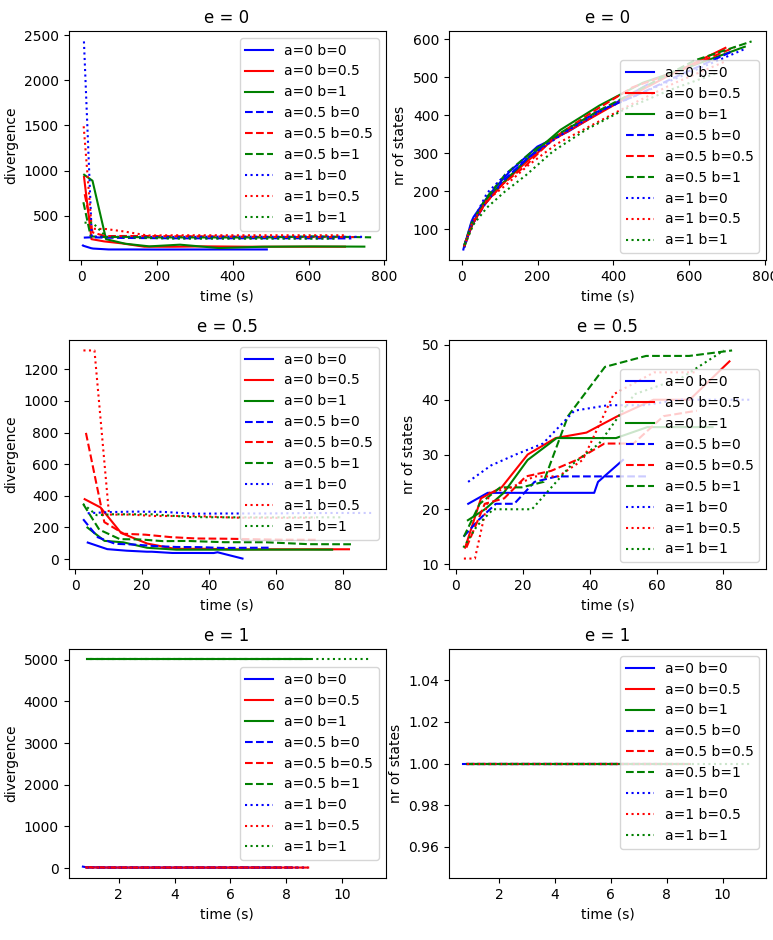
\includegraphics[width=0.7\columnwidth]{big_exp.png}
\caption{Experiments with $5\times5$ building. $a$, $b$, and $e$ stand for $\alpha$, $\beta$, and $\epsilon$, respectively \label{fig:big_experiments}.}
\end{figure}

\end{frame}

\begin{frame}
\frametitle{Experimental Evaluation}

\begin{figure}
\centering
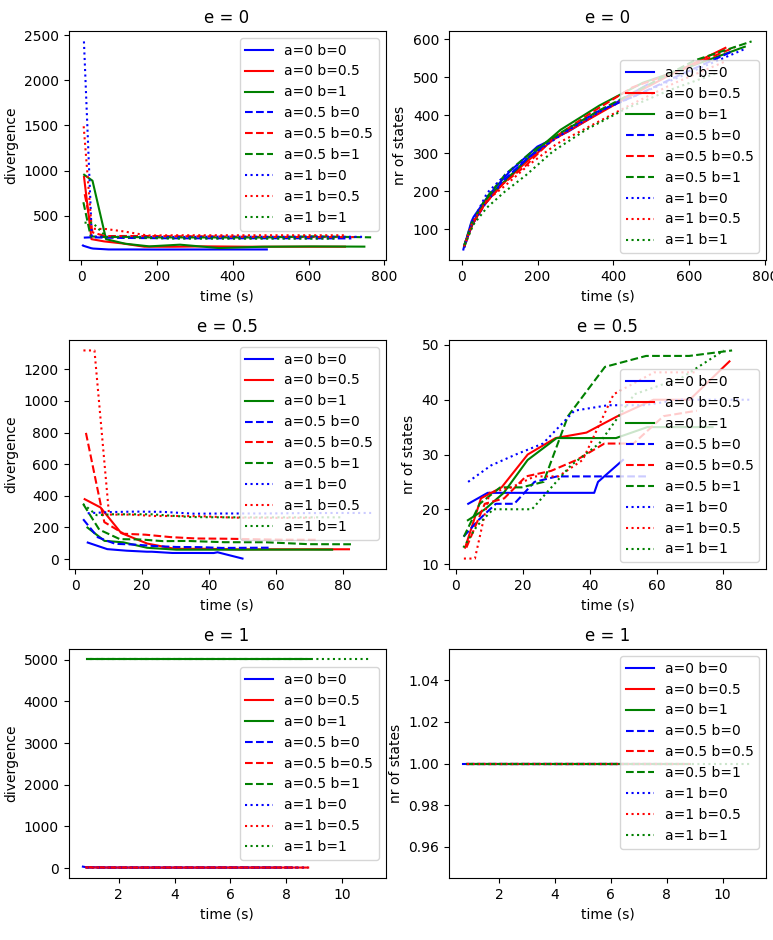
\includegraphics[width=\columnwidth]{big_exp.png}
\caption{Experiments with $5\times5$ building. $a$, $b$, and $e$ stand for $\alpha$, $\beta$, and $\epsilon$, respectively \label{fig:big_experiments}}.
\end{figure}

\end{frame}

\begin{frame}
\frametitle{Conclusions}

We have provided
\begin{itemize}
\item[$\bullet$]
A formal framework for the incremental 
construction of an abstract planning domain by learning new states
and the mapping between states and real world perceptions.
\item[$\bullet$]
A planning-acting-learning algorithm that allows an agent to learn
a coherent abstract planning model while planning and acting to achieve its
goals.
\end{itemize}

\pause
{\color {red}
Future Work:}
\begin{itemize}
\item[$\bullet$]
{\color {red}
Non-deterministic and Probabilistic (MDP) planning domains}
\item[$\bullet$]
{\color {red}
State merging and state elimination}
\item[$\bullet$] 
{\color {red} Imperfect sensors}
\item[$\bullet$] 
{\color {red} From abstract states to state variables}
\item[$\bullet$] 
{\color {red} Learning by Logic Tensor Network}
\end{itemize}

\end{frame}

\begin{frame}
  \begin{center}
    
\Large{
  {\color {red} {\bf THANK YOU FOR YOUR ATTENTION!}}}

  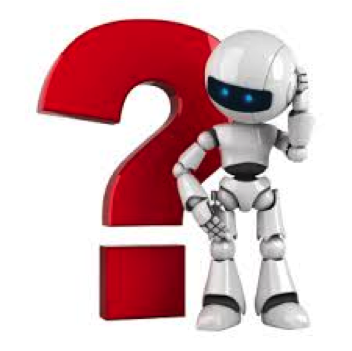
\includegraphics[width=.3\textwidth]{robot_quest.png}
  
\includegraphics[width=.3\textwidth]{robot_learned.jpg}
  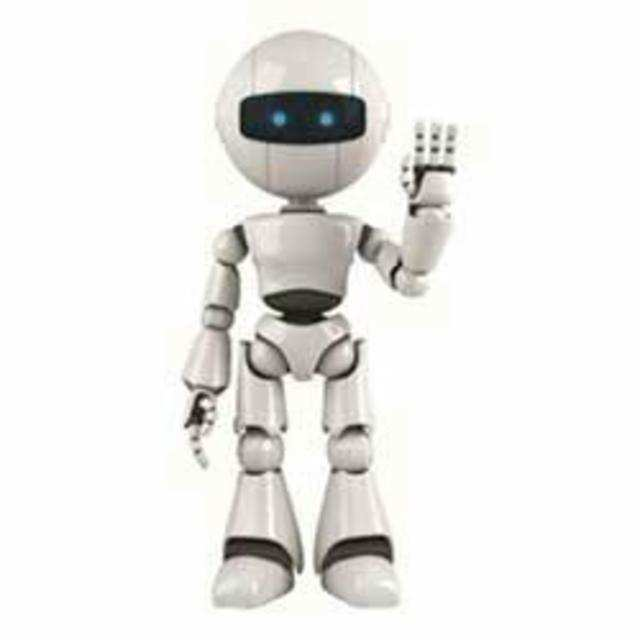
\includegraphics[width=.3\textwidth]{robot.jpg}
\end{center}
\end{frame}


\begin{frame}
  \begin{itemize}
  \item The agent is in state $s_0$ and has planned to execute $a$
  \item it executes $a$ and observes $\bx$
  \item it predicts to be in $\gamma(a,s)$, but according to the
    observations it is in the state
    % $$
    % s'=\argmax_s\left(\delta\cdot\mathbb{1}_{s=\gamma(a,s_0)}+\delta\cdot
    % \frac{f(\bx,s)}{\max f(\cdot,\cdot)}\right)
    % $$
    $$
    s'=\argmax_sf(\bx,s)
    $$
  \end{itemize}
\end{frame}
\begin{frame}
  \frametitle{Thanks for your attention}
  \begin{center}
  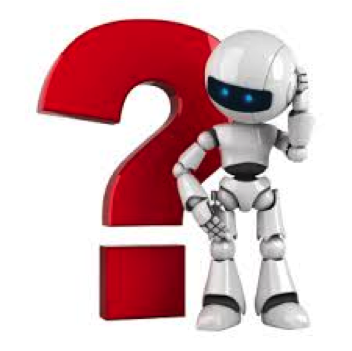
\includegraphics[width=.3\textwidth]{robot_quest.png}
  
\includegraphics[width=.3\textwidth]{robot_learned.jpg}
  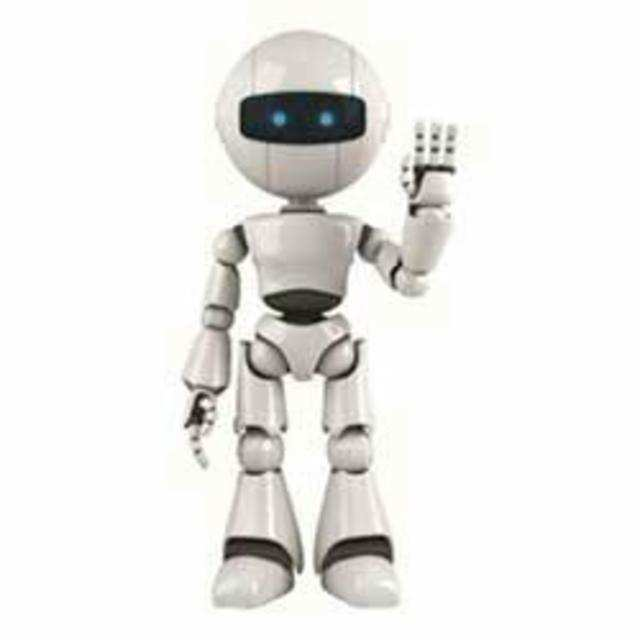
\includegraphics[width=.3\textwidth]{robot.jpg}
\end{center}
\end{frame}
\end{document}


if such a likelihood is below the threshold $(1-\epsilon)\cdot\max
p_{init}(\cdot)$ 
with $\epsilon \in [0,1]$, and where $p_{init}(\cdot)$ is the initialization function of 
the perception function, 
then we extend the set of states $S$ with a new state $s_{new}$, and
initialise its perception function $f(\cdot,s_{new})$ with
$p_{init}(\cdot)$ (lines 9--11). 
%
Notice that, low values of
$\epsilon$, promote the easy introduction of new states,
while with high values of $\epsilon$ we are cautious in
creating new states. In the extreme case, i.e., with $\epsilon=1$,
we never add new states. 

We then extend the sequence of transitions $\T$ and of observations $\O$, and learn the  new transition function $\gamma$ and the new perception function $f$. 
%
The functions $\updgamma$ and $\updf$ update the transition function
$\gamma$ and the perception function $f$, respectively, depending on
the data available in $\T$ and $\O$. The update functions take into
account (i) the current model, (ii)
what has been observed in the past, i.e., $\T$ and $\O$, and (iii)
what has been just observed, i.e., $\left<s_0,\pi(s_0),s_0'\right>$
and $\left<s_0',\bx\right>$.
%
% \subsection{Updating the model}
The update functions can be defined in several different ways, depending
on whether we follow a cautious strategy, where changes are made only
if there is a certain number of evidences from acting and perceiving
the real world, or a more impulsive reaction to what the agent has
just observed.
% 
% There are three components of the planning domain that need to be
% updated, namely: the set of states $S$, the transition function
% $\gamma$, and the perception function $f$. The level of cautiousness
% of the three updates applied by the agent, is encoded in three parameters, namely,
% $\epsilon$, $\alpha$ and $\beta$, all varying in the $[0,1]$
% interval. A $0$ value means no caution in update, and value $1$ means no
% update at all.

% \paragraph{Updating the set of states.}
% We assume that action executions cause observations that result in a vector  
% $\bx$ in $\R^n$. The \PAL\ algorithm determines
% the abstract state that maximize the likelihood of the
% observation $\bx$, i.e., it computes $\argmax_{s\in S}f(\bx,s)$ (line
% 7). 
% {\color {red}
% RIPETIZIONE, VEDI SU
% When the maximum likelihood is below a certain threshold,
% i.e $(1-\epsilon)\cdot\max p_{init}(\cdot)$, this means that the agent
% is not sufficiently confident to be in any of its known states, 
% and therefore, it extends the set of states by
% introducing a new state $s_{new}$, and initializes $f(\cdot,s_{new})$
% with the initialization perception function $p_{init}(\cdot)$.
% Notice that, when $\epsilon$ is
% close to $1$, the agent will rarely introduce new states, this
% corresponds to the fact that the agent is self confident about its
% abstract representation. While with low values of $\epsilon$ the
% agent will introduce new states, for almost all the observations,
% which means that it believes that its representation is too poor and
% needs to be extended to cope with every new observation.
% }

\noindent
\textbf{Updating transitions:}
$\updgamma$ decides whether and how to update the transition function.
Suppose that, after executing the action $a$ from the state $s_0$,
the agent perceives $\bx$, and suppose that
$s'_0=\argmax_{s}(f(\bx,s))$,
i.e., the most likely reached state, 
is different from the state predicted by the agent planning domain,
i.e., $s'_0\neq \gamma(a,s_0)$, then $\gamma$ may need to be revised to take into account this discrepancy. 
Since our domain is deterministic (the transition $\gamma$ must lead
to a single state), if the execution of an action leads to an
unexpected state, we have only two options: either change $\gamma$
with the new transition or not. 
We propose the following transition update function that
depends on $\alpha$: 
% expressing the agent tendency
% to be cautious or brave in the update of its planning domain:
We define 
$\updgamma(\gamma,\T)(s,a)=s'$  where $s'$ is \emph{one element}%
\footnote{To extend $\updgamma$ for nondeterministic domains, we could
  select a subset of states instead of a single one depending on the
  value of $\alpha$. The generalization to probabilistic domains would
  require to change the probability distribution on $\gamma$. In this
  paper we focus on deterministic domains.}
of the set
\begin{equation}
\{\argmax_{s'\in S}\left(\alpha\cdot\mathbb{1}_{s'=\gamma(s,a)}+
    (1-\alpha)\cdot|\{i\mid \T_i=\left<s,a,s'\right>\}|
\right)\}
\label{eq:upd_gamma}
\end{equation}
where $\mathbb{1}_{s'=\gamma(s,a)}$ is equal to 1 if
$s'=\gamma(s,a)$ and $0$ otherwise, $\T_i$ is the $i$-th element of
$\T$, and $\alpha\in[0,1]$. 
Notice that, if
$\alpha = 1$, we are extremely cautious, we strongly believe in our
model of the world, and we never change the transition $\gamma$.
Conversely, if $\alpha = 0$, we are extremely impulsive, we do not trust our model,
and just one evidence makes us to change the model. In the
intermediate cases, $\alpha \in (0,1)$, depending on the value of
$\alpha$, we need more or less evidence to change the planning
domain.

\noindent
\textbf{Updating the perception function:}  
The update of the perception function is based on the current
perception function $f(\bx,s)$ for $s\in S$ and the set of
observations $\O$. We suppose that the perception function is parametric on
$\prm=\left<\theta_1,\dots,\theta_k\right>$. In Example~\ref{ex:simple}, $\prm=\langle\theta_1,\theta_2\rangle$ with $\theta_1=\bmu$ and $\theta_2=\bSigma$, i.e., the mean and the covariance
matrix of the normal distribution associated to any state.
%
Given a new observation $\left<\bx,s\right>$ and a set of previous
observations $\O(s)=\left<\bx^{(0)},\dots, \bx^{(k)}\right>$ about an
abstract state $s\in S$, we have to update the parameters $\prm_s$ of
the perception function $f(\cdot,s)$ in order to
maximize the likelihood of the entire set of observations extended
with the new observation. Also in this case the agent can be more or less
careful in the revision. This is expressed by a parameter
$\beta\in[0,1]$, where, the higher the value of $\beta$ the
more careful the agent is in
the revision. If $f(\bx,s) = p(\bx|s,\prm_s)$, we define
$\updf(f,\O)(\bx,s)$ as 
$p(\bx\mid s,\prm'_s))$
where: 
\begin{align}\small
  \label{eq:update-f}
  \prm'_s & = \beta\cdot\prm_s+(1-\beta)\cdot
            \argmax_{\prm''} \mathcal{L}(\prm_s'',\O(s),\bx,s)
\end{align}
where 
$\mathcal{L}(\prm,\bx^{(1)},\dots,\bx^{(n)},s)$ 
is the likelihood of the 
parameters $\prm$ for the observations $\bx^{(1)},\dots,\bx^{(n)}$,
defined as: 
\begin{align}
  \label{eq:max-like-prm}
\mathcal{L}(\prm,\bx^{(1)},\dots,\bx^{(n)},s) & = 
  \prod_{i=1}^nP(\bx^{(i)}|s,\prm)
\end{align}
Intuitively Equation \eqref{eq:update-f} defines the parameters
$\prm'_s$ of the updated perception function for a state $s$ as a
convex combination, based on the parameter $\beta$, of the parameters
of the previous perception function for $s$, i.e., $\prm_s$ and the
parameters $\prm''$ that maximize the likelihood of the past and
current observations about state $s$ (equation
\eqref{eq:max-like-prm}).  An efficient procedure for incremental
estimation of the second term of \eqref{eq:update-f}, is described in
\cite{bishop2006}. In case of Multivariate Gaussian distribution,
$\prm_s$ contains the mean $\bmu_s$ and covariance matrix $\bSigma_s$,
and the updates defined in equation \eqref{eq:update-f} can be
efficiently computed as follows:
\begin{align*}
  \bmu'_s & = \beta\cdot\bmu_s+(1-\beta)(\bmu_s + \Delta\bmu_s) \\
  \bSigma'_s & = \beta\cdot\bSigma_s+(1-\beta)(\bSigma_s + \Delta\bSigma_s) \\
\end{align*}
where $\Delta\bmu_s=\frac{1}{|\O(s)|}(\bx-\bmu_s)$
and $\Delta\bSigma^2_s = \frac{1}{|O(s)|}(\bx-\bmu_s')^2 +
\frac{|O(s)|-1}{|O(s)|}(\Delta\bmu_s^2-2\bmu_s\Delta\bmu_s) -\frac{1}{|O(s)|}\bSigma^2_s$.
Concerning the parameter $\beta\in[0,1]$, it plays the similar role
as $\alpha$ in the case of the revision of the transition function.
It balances the update depending on whether the agent is cautious or impulsive
about the current perception function, and the new perceptions. 


% To sum up, the agent can control the update of its planning domain and
% perception function by setting the three parameters, $\alpha$, $\beta$, and
% $\epsilon$.
% \begin{itemize}
% \item $\alpha$ controls the update of the transition function;
% \item $\beta$ controls the update of the perception function;
% \item $\epsilon$ controls the update of the set of states. 
% \end{itemize}
% All the parameters take values in $[0,1]$. High values 
% induce a cautious revision strategy, while low values allow for
% a more reactive revision. 

\begin{example} 
Let us now describe how our algorithm works in Example~\ref{ex:simple}
and how the goal is reached by creating new states and changing the
model to the one described in Figure~\ref{fig:pd_pf_w_rev}.
\begin{enumerate}
\item 
  Suppose that the robot is initially in the position $(0.5,0.5)$ and
  that, according to its perception function, it believes to be in
  $s_{11}$ (notice indeed that $s_{11}=\argmax_{s_{ij}}f((0.5,0.5),s_{ij})$
  when
  $f((x,y),s_{ij})=\N((0.5,0.5),\bmu=(i-0.5,j-0.5),
  \bSigma=\left(\begin{smallmatrix}1 & 0 \\ 0 & 1\end{smallmatrix}\right))$). 
\item (line 4)
According to the planning domain in Figure~\ref{fig:pd_pf_w}.(a), $Plan(\PP)$ 
can generate two plans, the one that reaches the goal passing through
$s_{21}$ and the one that passes through $s_{12}$. Let us suppose
that it generates the former, i.e., the plan $\pi(s_{11})=e$ and
$\pi(s_{21})=n$.

\item (line 6-7)
Since $\pi(s_{11})$ is defined, we execute the action $e$, which moves
the robot of one unit in the east direction, and returns the current
position in $\bx$, which will be some value close to
$\left<1.5,0.5\right>$. Notice that we cannot assume that $\bx$ is
exactly $\left<1.5,0.5\right>$, since we have to take into
consideration that sensors and actuators can be noisy. So suppose that
the observed values after the execution of $\pi(s_{11})$ are 
$\left<1.51,0.49\right>$. 
Given the current $f$, the state $s$ that maximizes 
$f(\bx,s)$ is $s_{21}$, therefore $s_0' = s_{21}$.
\item (lines 8,13,14)
  Suppose that the condition on line 8 is false. We then do not create a new state. 
%
We add the transition to the history and we have $\T = \langle \langle s_{11}, e, s_{21} \rangle \rangle$.
Similarly we have $\O = \langle \langle s_{21}, \langle 1.51,0.49\rangle \rangle$. 
\item (lines 15) We then update the transition function: $\updgamma$
  does not produce any change, since $s_{21} =
  \gamma(s_{11},e)$. Indeed in this case the transition function
  $\gamma$ correctly predicts, at the abstract level, the effects of
  the execution of action $e$ in state $s_{11}$.

\item (line 16) The update of the perception function will
slightly move the mean $\bmu$, from $\left<1.5,0.5\right>$ in the
  direction of the current perception i.e., $\left<1.51,0.49\right>$
  and the $\bSigma$ will also be updated. 
\item We then update $s_0'$ to $s_{21}$ and go back to (lines 3,4).
Since $\pi(s_{21})=n$, 
%we don't need to replan
we execute the action moving one unit north from $s_{21}$. 
But the execution of this action does not have the effect that is expected by the agent, i.e., 
it does not reach state $s_{22}$. 
Indeed, the execution of $n$ starting from the position
$\left<1.51,0.49\right>$ would result in hitting the wall, 
the presence of which was not expected by the agent.
Let us suppose that the execution of this action will result in the robot
  doing nothing, and $act(\pi(s_{21}))$ will return the value $\bx$
  which is the same as the previous one i.e.,
  $\bx=\left<1.51,0.49\right>$. 
\item $s_{21}$ is the state that maximizes the observed
  $\bx$, and we proceed as before, by not generating a new state and
  appending the new transition to $\T$ such that
  $\T = \langle 
  \langle s_{11}, e, s_{21} \rangle,
  \langle s_{21}, n,  s_{21} \rangle \rangle$
  while $\O$ becomes
  $\langle
  \langle s_{21}, \langle 1.51,0.49\rangle\rangle,
  \langle s_{21}, \langle 1.51,0.49\rangle\rangle
  \rangle
  $
\item (line 15) The transition function this time gets updated in different
  ways depending on the value of $\alpha$.
  Let's compute the arguments of the argmax of equation 
  \eqref{eq:upd_gamma} with $a=n$ and $s=s_{21}$;
  $$\small 
  \begin{array}{|l|l|}\hline
    s' & \alpha\cdot\mathbb{1}_{s'=\gamma(s_{21},n)}+
         (1-\alpha)\cdot|\{i\mid \T_i=\left<s_{21},n,s'\right>|\\
    \hline 
    s_{11} & \alpha\cdot 0 + (1-\alpha)\cdot 0 = 0 \\
    s_{21} & \alpha\cdot 0 + (1-\alpha)\cdot 1 = (1-\alpha)\\
    s_{12} & \alpha\cdot 0 + (1-\alpha)\cdot 0 = \alpha\\
    s_{22} & \alpha\cdot 1 + (1-\alpha)\cdot 0 = 0 \\ \hline              
  \end{array}
  $$
If $\alpha < 1/2$, 
we are reasonably keen to learn from acting in the
real world that the state that maximizes equation \eqref{eq:upd_gamma} is $s_{21}$
and $\updgamma$ deletes $\gamma(s_{21},n) = s_{22}$ and adds
$\gamma(s_{21},n) = s_{21}$, i.e., the agent understands that there is
a wall that does not allow the robot to move north from state
$s_{21}$.
If instead $\alpha > 1/2$, then the state that maximizes \eqref{eq:upd_gamma}
is $s_{22}$ and $\gamma(s_{21},n)=s_{22}$ will be
kept. Notice that after $k$ attempts to execute the actions $n$ in
state $s_{21}$ without updating the transition function, in order to
change the transition function it is enough to have $\alpha <
\frac{k}{1+k}$. So if $\alpha\neq 1$, sooner or later the agent will
update $\gamma$. 
\item At this point we go back to $Plan(\PP)$ which generates the
  alternative plan that passes through $s_{12}$, and sends the robot
  back to state $s_{11}$ and then to state $s_{12}$, in a similar way
  to what happened in the case of going through $s_{21}$.
\item At this point the planning domain of the agent is shown
  below. Notice that the goal is not reachable. 
\begin{center}
  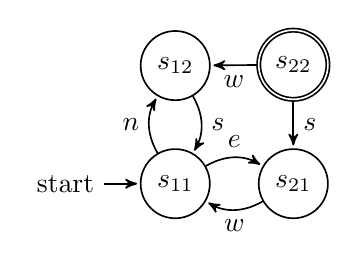
\begin{tikzpicture}[->,>=stealth',shorten >=1pt,auto,node distance=.6cm,
                    semithick,  baseline=(current bounding box.center)]
                    \node[initial,state] (s11) {$s_{11}$};
\node[state,above = of s11] (s12) {$s_{12}$};
\node[state,right = of s11] (s21) {$s_{21}$};
\node[state,accepting,above = of s21] (s22) {$s_{22}$};
\path (s11) edge [bend left] node {$e$} (s21)
            edge [bend left] node {$n$} (s12)
      (s12) edge [bend left] node {$s$} (s11)
      (s21) edge [bend left] node {$w$} (s11)
      (s22) edge node {$w$} (s12)
            edge node {$s$} (s21);            
     \end{tikzpicture} 
\end{center}
        
\item After having explored all the possibilities without reaching the
  goal, $Plan(\PP)$ generates random (exploration) plans. Suppose that
  it generates a plan $\pi$ with $\pi(s_{21})=e$. The observation
  after the execution of such a $\pi$ returns
  $\bx = \langle x,y \rangle$ close to $\left<2.5,0.5\right>$.  In
  that position $s_{21}$ maximises $f(\bx,s)$, however the value of
  $f(\bx,s_{21})$ is extremely low, and let us suppose it is below the
  threshold $(1-\epsilon)\cdot \max p_{init}(\cdot)$. We therefore create a new
  state, say $s_{31}$.
\item 
$\T$ gets updated by adding the transition 
$\langle s_{21},e,s_{31} \rangle$, and $\O$ by adding 
the pair $\langle s_{31}, \bx \rangle$.
%
The update function $\updgamma$ may create the new transition
$\gamma(s_{21},e) = s_{31}$ (if $\alpha$ is small enough) and $\updf$ 
will initialize the perception function $f(\cdot,s_{31})$ with
$p_{init}\sim\N(\bmu,\bSigma)$ with $\bmu=\bx$, and
$\bSigma=\left(\begin{smallmatrix}.1&0\\0&.1\end{smallmatrix}\right)$. 
\item
The next step is similar to the previous one.
Since there is no plan to the goal, $plan(\PP)$ tries to learn the domain, and state $s_{32}$ is created, transition $\gamma(s_{31},n)$  and the corresponding $f$ are created. Since no plan to the goal exists yet, while trying to learn the domain,
$plan(\PP)$ may add the new transitions $\gamma(s_{31},w)=s_{21}$ and $\gamma(s_{32},s)=s_{31}$ 
\item
In the final step, $plan(\PP)$ learns the transition
$\gamma(s_{32},w)=s_{22}$, and finally finds the plan to the goal
$\pi(s_{32}) = w$. Furthermore, the agent has
updated its initial planning domain, obtaining the planning domain
shown in Figure~\ref{fig:pd_pf_w_rev}.
Notice that this planning
domain is not completely correct, as there are no information about the execution of actions in $s_{22}$. This is due to the fact that, in this simple example, the agent has planned no
actions in $s_{22}$ (since it was the goal) and therefore it has not
learned anything about the transitions and the perceptions functions
of this node. 
\end{enumerate}
%
\begin{figure}
  \begin{center}
%  \begin{tabular}{cc}
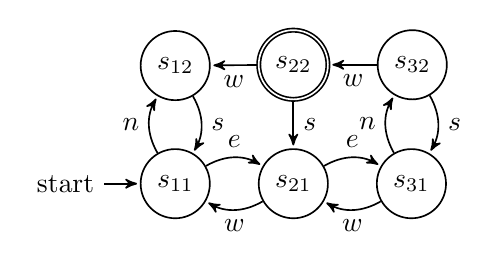
\begin{tikzpicture}[->,>=stealth',shorten >=1pt,auto,node distance=.6cm,
                    semithick,  baseline=(current bounding box.center)]
\node[initial,state] (s11) {$s_{11}$};
\node[state,above = of s11] (s12) {$s_{12}$};
\node[state,right = of s11] (s21) {$s_{21}$};
\node[state,accepting,above = of s21] (s22) {$s_{22}$};
\node[state,right = of s21] (s31) {$s_{31}$};
\node[state,right = of s22] (s32) {$s_{32}$};
\path (s11) edge [bend left] node {$e$} (s21)
            edge [bend left] node {$n$} (s12)
      (s12) edge [bend left] node {$s$} (s11)
%            edge [loop left] node {$n,w$} (s12)
      (s21) edge [bend left] node {$e$} (s31)
            edge [bend left] node {$w$} (s11)
%            edge [loop below] node {$s,n$} (s21)
      (s22) edge node {$w$} (s12)
            edge node {$s$} (s21)
      (s31) edge [bend left] node {$w$} (s21)
            edge [bend left] node {$n$} (s32)
%            edge [loop below] node {$s,e$} (s21)
      (s32) edge node {$w$} (s22)
%             edge [loop left] node {$n,e$} (s32)
            edge [bend left] node {$s$} (s31);
experiments
      \end{tikzpicture} 
% \begin{tikzpicture}[scale=.4,baseline=(current bounding box.center)]
%   \begin{axis}[view={0}{90},
%     colormap/hot,
%     xmin = 0,
%     xmax = 3,
%     ymin = 0,
%     ymax = 2,
%     axis equal image,
%     samples=5,
%     domain=0:2,
%     y domain=0:2,
%     ]
%    \def\centerx{.5}
%    \def\centery{.5}
%     \addplot3[contour gnuplot,domain=-2:6,domain y=-5:3] 
%         {10*exp(-10*( (x-\centerx)^2 + (y-\centery)^2)/3 )};
%    \def\centerx{1.5}
%    \def\centery{.5}
%     \addplot3[contour gnuplot,domain=-2:6,domain y=-5:3] 
%         {10*exp(-10*( (x-\centerx)^2 + (y-\centery)^2)/3 )};
%    \def\centerx{1.5}
%    \def\centery{1.5}
%     \addplot3[contour gnuplot,domain=-2:6,domain y=-5:3] 
%         {10*exp(-10*( (x-\centerx)^2 + (y-\centery)^2)/3 )};
%    \def\centerx{.5}
%    \def\centery{1.5}
%     \addplot3[contour gnuplot,domain=-2:6,domain y=-5:3] 
%         {10*exp(-10*( (x-\centerx)^2 + (y-\centery)^2)/3 )};
%    \def\centerx{2.5}
%    \def\centery{1.5}
%     \addplot3[contour gnuplot,domain=-2:6,domain y=-5:3] 
%         {10*exp(-10*( (x-\centerx)^2 + (y-\centery)^2)/3 )};
%    \def\centerx{2.5}
%    \def\centery{0.5}
%     \addplot3[contour gnuplot,domain=-2:6,domain y=-5:3] 
%         {10*exp(-10*( (x-\centerx)^2 + (y-\centery)^2)/3 )};
%       \end{axis}
%     \end{tikzpicture}
     %    \end{tabular}
\end{center}      
  \caption{\label{fig:pd_pf_w_rev} The new planning domain
    obtained by extending the initial domain of Figure~\ref{fig:pd_pf_w},
    with two new states}
\vspace*{-10pt}
\end{figure}
\end{example}

\section{Measuring the coherence of the model}
In order to estimate the quality of the model generated by the \PAL\
algorithm, we should define a method to measure the coherence between
an abstract model with perception function and the real world.

We introduce a measure called \emph{divergence}. 
Intuitively, a low divergence means that if
$\gamma(a,s) = s'$, then if the agent perceives to be in $s$ and
performs $a$, then after the execution of $a$ it will perceive to
be in the state $s'$.

We suppose to have a stochastic model of the real execution of actions. 
Under Markovian hypothesis, every action $a \in A$ can be
modeled as a conditional PDF $p_a(\bx'|\bx)$,
which expresses the probability of measuring $\bx'$ after executing the action $a$ in a
state in which the agent perceives $\bx$. 
It represents
the effects of executing the action $a$ in the real world.

To measure the quality of the abstract planning domain, 
we have to compare $p_a$ with how
the action $a$ is modeled in the domain. 
%
Suppose that an agent perceives $\bx$, and that the state $s$
maximizes the likelihood of perceiving $\bx$. 
Suppose that the action $a$ is executed.
According to its abstract model, the agent will believe to be in
the state $s'=\gamma(a,s)$.
After the actual execution of action $a$, it will perceive $\bx'$
with a probability $p_a(\bx'|\bx)$. 
However, according to the agent's abstract model, 
the probability of observing $\bx'$ after the execution
of $a$ is $p(\bx'|s')$. 
The closer the two distributions are, 
the more coherent the abstract representation is. 
To estimate how well $p(\bx'|s')$ approximates the real distribution $p_a(\bx'|\bx)$, we
use the notion of  {\em divergence}, which is the opposite notion of coherence
(the lower the divergence, the higher the coherence), 
and we formalize it  with the 
{\em KL divergence} 
$KL(p_a(\bx'|\bx)||p(\bx'|s'))$,
defined as: 
$$
\int_{\bx'}p_a(\bx'|\bx)\log\left(\frac{p_a(\bx'|\bx)}{p(\bx'|s')}\right)\:d\bx'
$$
We can therefore define the divergence measure as
\begin{align}
  \label{eq:coherence}
  \int_{\bx}\sum_{a\in
  A}\mathrm{KL}(p_a(\bx'|\bx)||p(\bx'|\gamma(a,s_{\bx})))\cdot p_A(\bx)\: d\bx
\end{align}
where $s_{\bx}=\argmax_{s\in  S}f(\bx,s))$ and $p_A(\bx)$ is a distribution of all the possible perceptions
that can be obtained by the agent following all the possible sequences
of actions, i.e., 
$$
p_A(\bx)=\sum_{\left<a_1.\dots,a_n\right>\in A^+}p_{a_n}(\bx|\bx^{(n-1)})\cdot\prod_{i=1}^{n-1}p_{a_i}(\bx^{(i)}|\bx^{(i-1)})
$$
\def\ba{\mathbf{a}}
%
where $A^+$ is the set of finite non empty sequences of actions in $A$
and $\bx^{(0)}$ is the perception of the agent in the initial state. 
However, computing \eqref{eq:coherence} analytically is very difficult.
%
We therefore
estimate \eqref{eq:coherence} by random walk sampling method. Starting
from an initial observation $\bx^{(0)}$ we generate $N$ random
walks $\ba_1,\dots,\ba_N$, with
$\ba_i=\langle a_{i,1},\dots,a_{i,n_i}\rangle$ and sample $\bx^{(i)}$
from $\prod_{j=1}^{n_i}p_{a_{ij}}(\bx_{j}|\bx_{j-1})$. 
We approximate \eqref{eq:coherence} with
\begin{align}
  \label{eq:coherence-approx}
\frac{1}{N}\sum_{k=1}^N\sum_{a\in A}\mathrm{KL}(p_a(\bx'|\bx^{(k)})|| p(\bx'|\gamma(a,s^{(k)})))
\end{align}
where $s^{(k)} = \argmax_{s\in S}f(\bx^{(k)},s)$ for $1\leq k \leq
n$. 
In our specific example, since we are working with Gaussian
distributions, we have that 
%
$p_a(\bx'|\bx) =
\N(\bmu=a(\bx),\bSigma=\bSigma_a)$,
%
where $a(\bx)$ 
is some real function that maps  
$\bx$ in the expected value $a(\bx)$ after performing the action $a$, and $\bSigma_a$ is the model of the noise of the
sensors/actuators associated to $a$. For instance, in Example~\ref{ex:simple}
$$
e(\langle x,y\rangle)=
\begin{cases}
  \langle x+1,y\rangle & \parbox[t]{.3\textwidth}{If there are no walls
    between \\ $\left<x,y\right>$ ad $\left<x+1,y\right>$} \\
    \langle x,y\rangle & \mbox{Otherwise}
  \end{cases}
  $$
Furthermore, the KL divergence of Multivariate Gaussians can be
computed analytically. 

% using the following equation 
% \begin{equation}
%   \begin{split}
% & \frac{1}{2}\biggl( 
%   \log\frac{|\bSigma_{\gamma(a,s)}|}
%     {|\bSigma_{a}|}-d+tr(\bSigma_{\gamma(a,s)}^{-1}\bSigma_{a})
%      \\
%     &  \quad +(\bmu_{\gamma(a,s)}-a(\bx))^{\mathsf{T}}\bSigma_{\gamma(a,s)}^{-1}(\bmu_{\gamma(a,s)}-a(\bx))\biggr)
% \end{split}
% \end{equation}
% where $d$ is the dimension of $\bx$.


\section{Experimental Evaluation}

To explain and evaluate \PAL\ and its effects depending on different
parameter settings,
we propose two sets of experiments. We first run
\PAL\ on Example \ref{ex:simple} and successively we run the algorithm
on a larger artificial test case%
\footnote{The code is available in the additional material.}.
Since the paper does not focus on a specific plan generation
technique, we implement our approach using a naive planner, which uses an
heuristic based on the distance from the goal.

In the first experiment, the initial planning
domain is shown in Figure~\ref{fig:pd_pf_w} and, for different
configurations of the parameters $\alpha$, $\beta$, and $\epsilon$ in
$\{0.0,0.5, 1.0\}$, we run the \PAL\ algorithm 10 times. We measure
the average number of states of the final model ($|S|$), the
reduction/improvement of the divergence (``\% lrn") and the percentage of
achieved goals (\%G). The results are reported in table
~\ref{fig:explanatory-exp-eval}%
\footnote{The reviewer/reader
  interested to graphically see the computation of \PAL\ on this
  simple example with different parameters can download the additional
  material and run the command \texttt{python PALex1.py <alpha> <beta>
    <epsilon>}}.
%
Consider first the effects of the parameter $\epsilon$:
\begin{itemize}
\item $\epsilon = 1$ prevents the creation of new states. Indeed, in all cases, 
%if $\epsilon = 1$ 
no new state is created, and, as expected, the learned model is not more coherent than the initial one - the percentage of learning ``\% lrn'' ranges from a negative number ($-11.7$) to very low improvement ($0.26$).  Indeed, without
  creating new states, \PAL\ never understands that there are new
  rooms.  Because of this lack of coherence, in many cases \PAL\ does
  not manage to reach the goal within the given timeout (100 steps).
  The reason why in some cases it manages to reach the goal is simply
  due to the fact that, when no plan exists according to the model,
  then a random policy is tried, which in some cases reaches the goal
  by chance, due to the simple and small domain.
\item $\epsilon = 0$  tends to create many new states:
  $|S| \in [20.2,32.9]$.  In spite of this, when $\alpha = 0$, the
  learning is much better than when no new states are created (``\%
  lrn" $\in [0.49,0.54]$) and the goal is often reached. The learning
  gets worse by increasing $\alpha$, since we learn many new states
  that are however scarcely connected to the states in the initial
  model.
\item $\epsilon = 0.5$ represents a balanced situation.  The number of
  new learned states is the right one ($|S| \approx 6$) for all the
  values of the other parameters.  Moreover, with $\alpha = 0$ we have
  the best learning of a coherent model (``\% lrn $= 0.72$)), since
  we allow the update of the transition function by connecting the two
  new states with the four initial ones.  The performance of learning
  smoothly decreases by increasing $\alpha$ to $0.5$, while it becomes
  low in the case of $\alpha = 1$, due to the fact that the new states are not connected with the old ones. 
\end{itemize}
%
In the case $\alpha = 0$ and $\alpha = 0.5$, the parameter $\beta$,
when it is low ($\beta = 0$), tends to decrease the amount of learning
towards a coherent model, by producing the two worst results (``\%
lrn" $=-11.17$ and $-4.71$) in the case $\epsilon = 1$. This is
because, since we cannot learn new states, with a low $\beta$ we allow
the perception function to move the same old states to different
positions, thus creating a rather incoherent model.
\begin{table}[t]\footnotesize
\centering
\def\toprule{\hline}
\def\midrule{\hline\hline}
\def\bottomrule{\hline}
\tabcolsep=3pt
\begin{tabular}{|l|l|r|r|r|r|r|r|r|r|r|}
\toprule
$\alpha$ & $\beta$ & 
\multicolumn{3}{|c|}{$\epsilon=0.0$} & 
\multicolumn{3}{|c|}{$\epsilon=0.5$} & 
\multicolumn{3}{|c|}{$\epsilon=1.0$} \\  \cline{3-11}
& & $|S|$ & \%lrn & \%G & 
$|S|$ & \%lrn & \%G & 
$|S|$ & \%lrn & \%G \\ \midrule
0.0 & 0.0 &          21.6 &        0.49 &           1.0 & 
                      6.0 &        0.72 &           0.7 & 
                      4.0 &       -4.71 &           0.1 \\
    & 0.5 &          24.7 &        0.50 &           0.9 & 
                      5.9 &        0.72 &           0.8 & 
                      4.0 &       -0.41 &           0.9 \\
    & 1.0 &          20.2 &        0.54 &           0.9 & 
                      5.9 &        0.72 &           0.7 & 
                      4.0 &        0.18 &           0.9 \\ 
0.5 & 0.0 &          25.8 &        0.19 &           1.0 & 
                      5.9 &        0.66 &           0.8 & 
                      4.0 &      -11.17 &           0.2 \\
    & 0.5 &          30.7 &        0.15 &           0.7 & 
                      5.9 &        0.69 &           0.8 & 
                      4.0 &        0.26 &           0.8 \\
    & 1.0 &          32.9 &        0.16 &           0.7 & 
                      6.0 &        0.63 &           0.8 & 
                      4.0 &        0.07 &           0.7 \\
1.0 & 0.0 &          25.0 &        0.15 &           0.9 & 
                      5.9 &        0.25 &           0.5 & 
                      4.0 &        0.01 &           0.1 \\
    & 0.5 &          24.4 &        0.18 &           0.8 & 
                      5.8 &        0.24 &           0.8 & 
                      4.0 &       -1.26 &           0.8 \\
    & 1.0 &          28.5 &        0.16 &           0.8 & 
                     6.0 &        0.27 &           1.0 & 
                      4.0 &        0.00 &           0.9 \\
\bottomrule
\end{tabular}
\caption{Performance of \PAL\ on Example~\ref{ex:simple} depending on
  $\alpha$, $\beta$, and $\epsilon$. Results are averaged on the 10
  runs. 
\label{fig:explanatory-exp-eval}}
\vspace*{-12pt}
\end{table}

In the second set of experiments, we consider a $5\times5$ building with
randomly generated walls%
\footnote{A picture of this world is reported in the
  additonal material.} completely unknown by the agent. Differently from the previous
experiments, we test the capability of \PAL\ to create a planning
domain from scratch, while it is trying to achieve 10 randomly
generated goals%
\footnote{The reader can see how the system works with the different
  parameters by downloading the system from the supplementary material
  and run \texttt{python PAL.py <alpha> <beta> <epsilon>
    <nr\_of\_goals>}.}.  We initialise the agent with a model
containing only two states, i.e., $S=\{s_0,s_{g_0}\}$.  The mean
$\bmu_{s_0}$ of the initial state is set to $\left<0.5,0.5\right>$,
the mean of $s_{g_0}$ of the perception function of $s_{g_0}$ is
randomly generated.  The covariance matrixes $\bSigma_{s_0}$ and
$\bSigma_{s_{g_0}}$ are initialized to
$\left(\begin{smallmatrix}.1&0\\0&.1\end{smallmatrix}\right)$.  The
objective of the agent is to reach the goal $s_{g_0}$, and
successively to reach other 9 goals $s_{g_1},\dots,s_{g_9}$, which are
also randomly generated. We run this experiment, for every combination
of $\alpha$, $\beta$, and $\epsilon$ in $\{0.0,\ 0.5,\ 1.0\}$.  In
Figure \ref{fig:big_experiments} we report the divergence (in the
three plots on the left of the figure) and the number of states that
are generated (in the three plots on the right) depending on the time
used by \PAL\ to plan, act and learn (the x axis), and depending on
the parameters $\alpha$, $\beta$, and $\epsilon$.  Notice that the
graphs have different scales, since with a uniform scale some of the
graphs would not be readable.

% \begin{itemize}
% \item
If $\epsilon = 1$, \PAL\ cannot add new states to the planning model,
  and therefore, planning is useless, and the agent adopts a random
  walk strategy. Furthermore, the divergence is computed only on a single
  state. The consequence is that $\alpha$ does not have any effect,
  since with a single state there is no transition to revise. 
  Instead, the value of $\beta$ has the effect of (dis)allowing the change of
  the perception function associated to the single state $s_0$. If
  $\beta=1$, the perception function  $f(\bx,s_0)$ is not changed and,
  consequently, the divergence is constant (i.e., it takes its initial 
  value $\approx 5000$); with $\beta\neq 1$, instead, the
  perception function $f(\bx,s_0)$ is updated to take into 
  account the observations that the agent accumulates
  during its random walk, but after short time it converges to a
  constant value $\approx 13.0$. 

%\item 
  If $\epsilon = 0$, \PAL\ tends to generate an eccessive number
  of states independently from $\alpha$ and $\beta$: We get to about $600$
  states in $800$ seconds. In this case \PAL\ learns a domain by
  decreasing significantly the divergence, which gets below $500$ for
  all the values of $\alpha$ and $\beta$. It takes however a long
  time to complete the tasks, up to 800 seconds, because the model is
  uselessly accurate. 
  
%\item
  If $\epsilon = 0.5$, \PAL\ generates a reasonable number of
  states.  For all the values of $\alpha$ and
  $\beta$, the completion of the task requires much less time than the
  case of $\epsilon = 0$.
  % Indeed, when we generate many states the model is much
  % more fine grained and planning is more expensive. 
  The best model, i.e., the one closest to our intuition, is the one
  generated in the case of $\epsilon = 0.5$, $\alpha = 0.5$, and
  $\beta = 0$. It has indeed 25 states, each one corresponding to the
  25 rooms in the building, and with transitions taking into account
  the walls.  In this case, the divergence rapidly decreases to values
  below 100.  Moreover, in all cases in which $\epsilon = 0.5$, we
  have divergences much lower than in the case $\epsilon = 0$ (please
  notice the different scale in the two graphs). Finally, we have
  lower divergences for low values of $\alpha$ ($\alpha = 0$ and
  $0.5$) than in the case of $\alpha = 1$, since, as usual,
  $\alpha = 1$ does not allow \PAL\ to connect the new states to the
  old ones.
% \end{itemize}

In conclusion, the experiments show that the new formal framework allows \PAL\ (with a very simple planning algorithm) to learn the abstract model (even from scratch) and, with a reasonable set up of the parameters, to learn coherent models in reasonable time. 
\begin{figure}
\centering
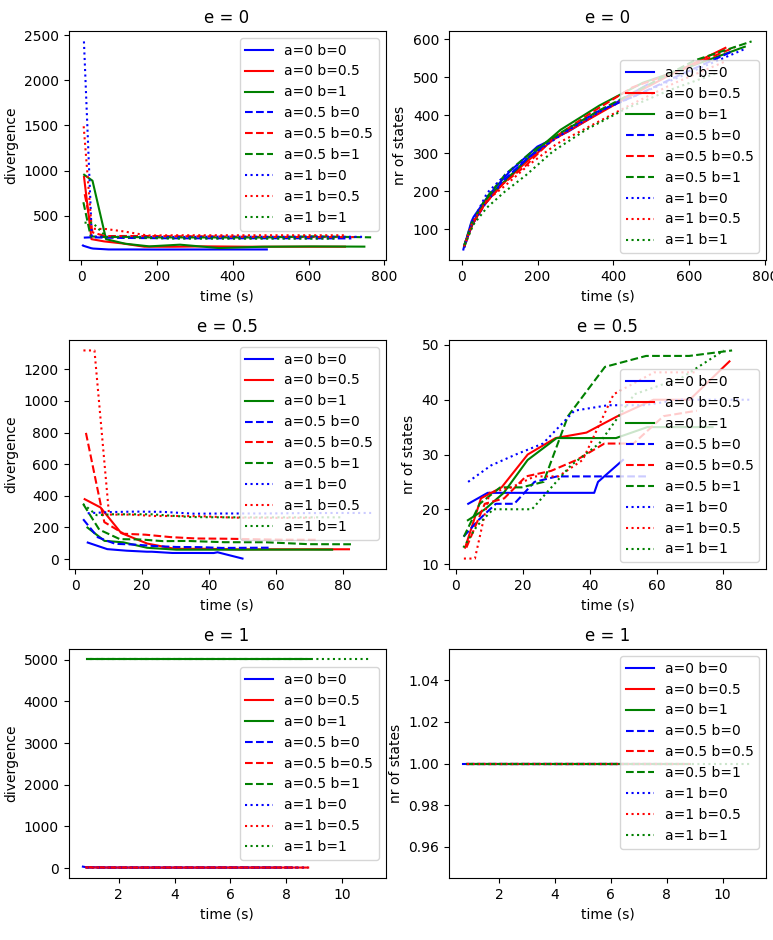
\includegraphics[width=\columnwidth]{big_exp.png}
\caption{Experiments with $5\times5$ building. $a$, $b$, and $e$ stand for $\alpha$, $\beta$, and $\epsilon$, respectively \label{fig:big_experiments}.}
\vspace*{-12pt}
\end{figure}
% \begin{figure}[t]
% \includegraphics[width=.5\textwidth]{learned_model.png}
% \caption{A 25 rooms building}
% \label{fig:big_model}
% \end{figure}

\section{Related Work}
\label{sec:rw}
Our approach shares some similarities with the work on planning by
model based reinforcement learning (RL)
\cite{kaelbling96,sutton98,geffner2013}, especially with approaches 
defined on abstract discrete models.
% Dyna \cite{sutton98} is one of the first systems
% integrating planning and model based reinforcement learning.
In \cite{yang2018} planning domains are specified in the action
language ${\mathcal BC}$ in a hierarchical reinforcement learning
setting.  In \cite{parr97} hierarchical abstract machines impose
constraints on reinforcement learning.  \cite{ryan2002} combines
symbolic planning techniques with reinforcement learning.  In
\cite{leonetti2016} plans are generated by answer set programming, and
reinforcement learning allows adaptation to a changing environment.
\cite{henaff2017,henaff2017ArXiv} adopts a different approach based on
model based planning to learn the planning domain directly from
execution traces.
%
All the works mentioned above assume that
the set of states and the correspondence between continuous data from
sensors and states are fixed a priori.  Furthermore, after acting, the
agent knows exactly the reached state. As a consequence there is no
possibility to learn a new state, or to learn to adapt the mapping
between perceptions in the real world and states. We, instead, allow
to introduce new states at run-time, and to adapt the perception
function.

% This main conceptual and practical difference with respect to our approach holds for the work integrating (symbolic) planning in an abstract model with reinforcement learning.
%
% Dyna \cite{sutton98} is one of the first systems integrating planning and model based reinforcement learning.
% % in which a reactive component chooses actions to be executed and Dyna computes a value function 
% % from both real experiences and simulated ones.
%
% In \cite{yang2018}, planning domains are specified in the action language ${\mathcal BC}$. The learning step enriches the planning domain specification.
%
% In \cite{parr97}, hierarchical abstract machines impose constraints on reinforcement learning.
% %
% In \cite{ryan2002}, symbolic planning techniques are combined with reinforcement learning.
% %
% In \cite{leonetti2016},  plans are generated by answer set programming, and reinforcement learning allows the planner to adapt to a changing environment. 
% %In \cite{zhang2017}, a declarative programming language with answer set semantics is used to reason about and  construct POMDP
% In all these works, while transactions from one state to another are learned, 
% the set of states of the abstract model (the signature of the domain) is fixed forever, never learned, and no mapping from a continuous space if formalized and learned.

% Beyond such main conceptual difference, there are some
% technical differences with the previously cited works. Most of them
% are related to the MDP framework.
% 
% A further technical difference with some of the cited works is that we
% do not necessarily start to learn from scratch the planning domain,
% but we start planning with an initial model of the world. This allows
% our approach to exploit a prior knowledge about the world rather than
% learning everything from scratch.
Moreover, we have explicit parameters like
$\alpha$ and $\beta$ in the $\updgamma$ and $\updf$ functions that we
can use to balance how much we trust in an initial model or
in the model learned so far. 

A complementary approach is pursued in works that plan directly in a
continuous space, see, e.g., \cite{abbeel2006,mnih2015,coeeyes2018}.
In this way there is no need to define a mapping such as the
perception function, since there is no abstract discrete model of the
world. Such approaches are very suited to address some tasks, e.g., moving a
robot arm to a desired position or performing some manipulations. 
However, we believe that, in several situations, it is
conceptually appropriate and practically efficient to perform planning
in an abstract discrete state space. 

Several approaches to planning for robotics (see Section 7 of
\cite{ingrand2017} for a comprehensive survey) deal with the problem
of planning in and learning the environment in which they operate, and
they have to deal with the robot ending up in unknown and unexpected
states of the world.  Some of them make use of an abstract model of
the world.
%
However, none of these works provide a formalization of the mapping
and of the learning mechanism as we provide in this paper.

Works on domain model acquisition focus on the different problem of
learning action schema, see,
e.g. \cite{gregory2016,mccluskey2009,cresswell2013,mourao2012,zhuo2013,mehta2011}.
%
Finally, our work has some similarities with planning in hybrid
domains (see, e.g., \cite{bogomolov2014}), since we deal with a
discrete model and continuous data coming from sensors. However we do
not plan in a hybrid domain, since our plan generation is performed in
the discrete space.

% Though our approach is limited to deterministic domains the extension
% to probabilistic can be done by suitably modifying the $\updgamma$ function, to
% increase or decrease the probabilities of transitions depending on the
% outcomes of actions.
%
% From the one side, a stochastic domain is more expressive than a
% deterministic one, since it allows for modeling uncertainty in action
% execution.
% %
% From the other side, plan generation is much simpler and more
% efficient in a deterministic domain than in a MDP framework, and we
% model uncertainty about the world by learning and updating the
% planning domain.


\section{Conclusion and Future Work}
\label{sec:conclusion}

We have provided a formal framework that supports the incremental 
construction of an abstract planning domain by learning new states
and the mapping between states and real world perceptions. We have
provided a planning-acting-learning algorithm that allows an agent to learn
a coherent abstract planning model while planning and acting to achieve its
goals. We have provided an experimental evaluation that shows how this
can be obtained with different learning modalities. 

In this paper we focus on deterministic domains; in the future we plan
to extend our work to nondeterministic and probabilistic planning
domains, e.g., by learning probability distributions on $\gamma$.
Moreover we plan to integrate in our framework a
state-of-the-art on-line planner, and to run experiments on more
complex and realistic domains.

\bibliographystyle{aaai}
\bibliography{biblio}
\end{document}



